\documentclass[conference]{IEEEtran}
\IEEEoverridecommandlockouts
\usepackage{cite}
\usepackage{amsmath,amssymb,amsfonts}
\usepackage{algorithm}
\usepackage{algpseudocode}
\usepackage{graphicx}
\usepackage{textcomp}
\usepackage{xcolor}
\usepackage{booktabs}
\usepackage{float}
\usepackage{url}
\usepackage{multirow}
\usepackage{hyperref}

\def\BibTeX{{\rm B\kern-.05em{\sc i\kern-.025em b}\kern-.08em
    T\kern-.1667em\lower.7ex\hbox{E}\kern-.125emX}}

\newcommand{\bx}{\mathbf{x}}
\newcommand{\bh}{\mathbf{h}}
\newcommand{\by}{\by}
\newcommand{\bz}{\mathbf{z}}

\begin{document}

\title{Neuro-Symbolic Safety Nets: Fusing Optimized Deep Learning with Interpretable Logic for Trustworthy Diagnosis}

\author{\IEEEauthorblockN{1\textsuperscript{st} Tomasz Karpiński}
\IEEEauthorblockA{\textit{Faculty of Physics and Applied Computer Science} \\
\textit{AGH University of Krakow}\\
Krakow, Poland \\
 tkarpinski@student.agh.edu.pl}
}

\maketitle

\begin{abstract} 
The "black box" nature of Deep Learning hinders its adoption in high-stakes medical domains. We propose a Hybrid Neuro-Symbolic Framework that fuses an optimized Multi-Layer Perceptron (MLP) with an interpretable symbolic expert layer. Using the CDC Diabetes Dataset, we implement a "Total Defense" strategy involving robust outlier detection (Isolation Forest) and rigorous Hyperparameter Optimization (HPO) via Optuna and Enhanced ALSHADE. Our system achieves a peak neural ROC-AUC of 0.82. While integrating the symbolic layer reduces discrimination (ROC-AUC 0.79), it acts as a critical safety audit, identifying 20.36\% of false negatives missed by data-driven models. This work demonstrates a viable path toward trustworthy, human-in-the-loop AI that prioritizes safety alongside accuracy.
\end{abstract}

\begin{IEEEkeywords}
Neuro-Symbolic AI, Hyperparameter Optimization, Explainable AI, Medical Diagnosis, Trustworthy AI, Autoencoders, Evolutionary Computing
\end{IEEEkeywords}

\section{Introduction}
Deep Learning offers high predictive accuracy but lacks the interpretability required for clinical trust. Purely data-driven models are often brittle, failing on edge cases without explanation. To bridge this "Trust Gap," we present a **Hybrid Neuro-Symbolic Diagnostic System** combining the statistical power of neural networks with transparent, logic-driven reasoning.

Our key contributions are:
\begin{enumerate}
    \item \textbf{Robust Preprocessing:} Evaluation of Isolation Forest \cite{cheng2019iforest} against standard Z-score pruning.
    \item \textbf{Hybrid Representation:} Comparison of raw features, PCA, and Autoencoder embeddings \cite{tschannen2018ae}.
    \item \textbf{Extensive Optimization:} Tuning of six optimizers (including Lion \cite{chen2023lion}) using Random Search, Optuna, and Evolutionary Algorithms (e.g., Enhanced ALSHADE \cite{karpinski2025deullm}).
    \item \textbf{Neuro-Symbolic Layer:} Integration of medical rules, fuzzy logic, and Bayesian updates to audit neural predictions.
    \item \textbf{Safety Analysis:} Demonstration that hybrid systems expose limitations of pure Deep Learning on difficult patient profiles.
\end{enumerate}

\section{Related Work}
While architectures like TabNet exist, MLPs remain effective for tabular data when properly regularized. Neuro-symbolic approaches often embed logic into training; our method uses a symbolic layer as an independent post-hoc auditor. We systematically compare HPO methods (Bayesian vs. Evolutionary) to optimize this neural baseline, contrasting with standard grid search approaches.

\section{Methodology}

\subsection{Dataset & Preprocessing}
We utilize the **CDC Diabetes Health Indicators Dataset**. To address the 1:7 class imbalance (Fig. \ref{fig:class_dist}), we implemented a "Total Defense" strategy:
1.  **Isolation Forest:** Removes anomalies based on feature splits rather than statistical tails (Fig. \ref{fig:outlier_comp}).
2.  **Random Oversampling:** Balances the minority class.
3.  **Weighted Loss:** \texttt{BCEWithLogitsLoss} prioritizes sensitivity.
4.  **Dynamic Thresholding:** Maximizes F1-Score on validation data.

\input{generated_tables/table_dataset_stats.tex}

\begin{figure}[htbp]
\centerline{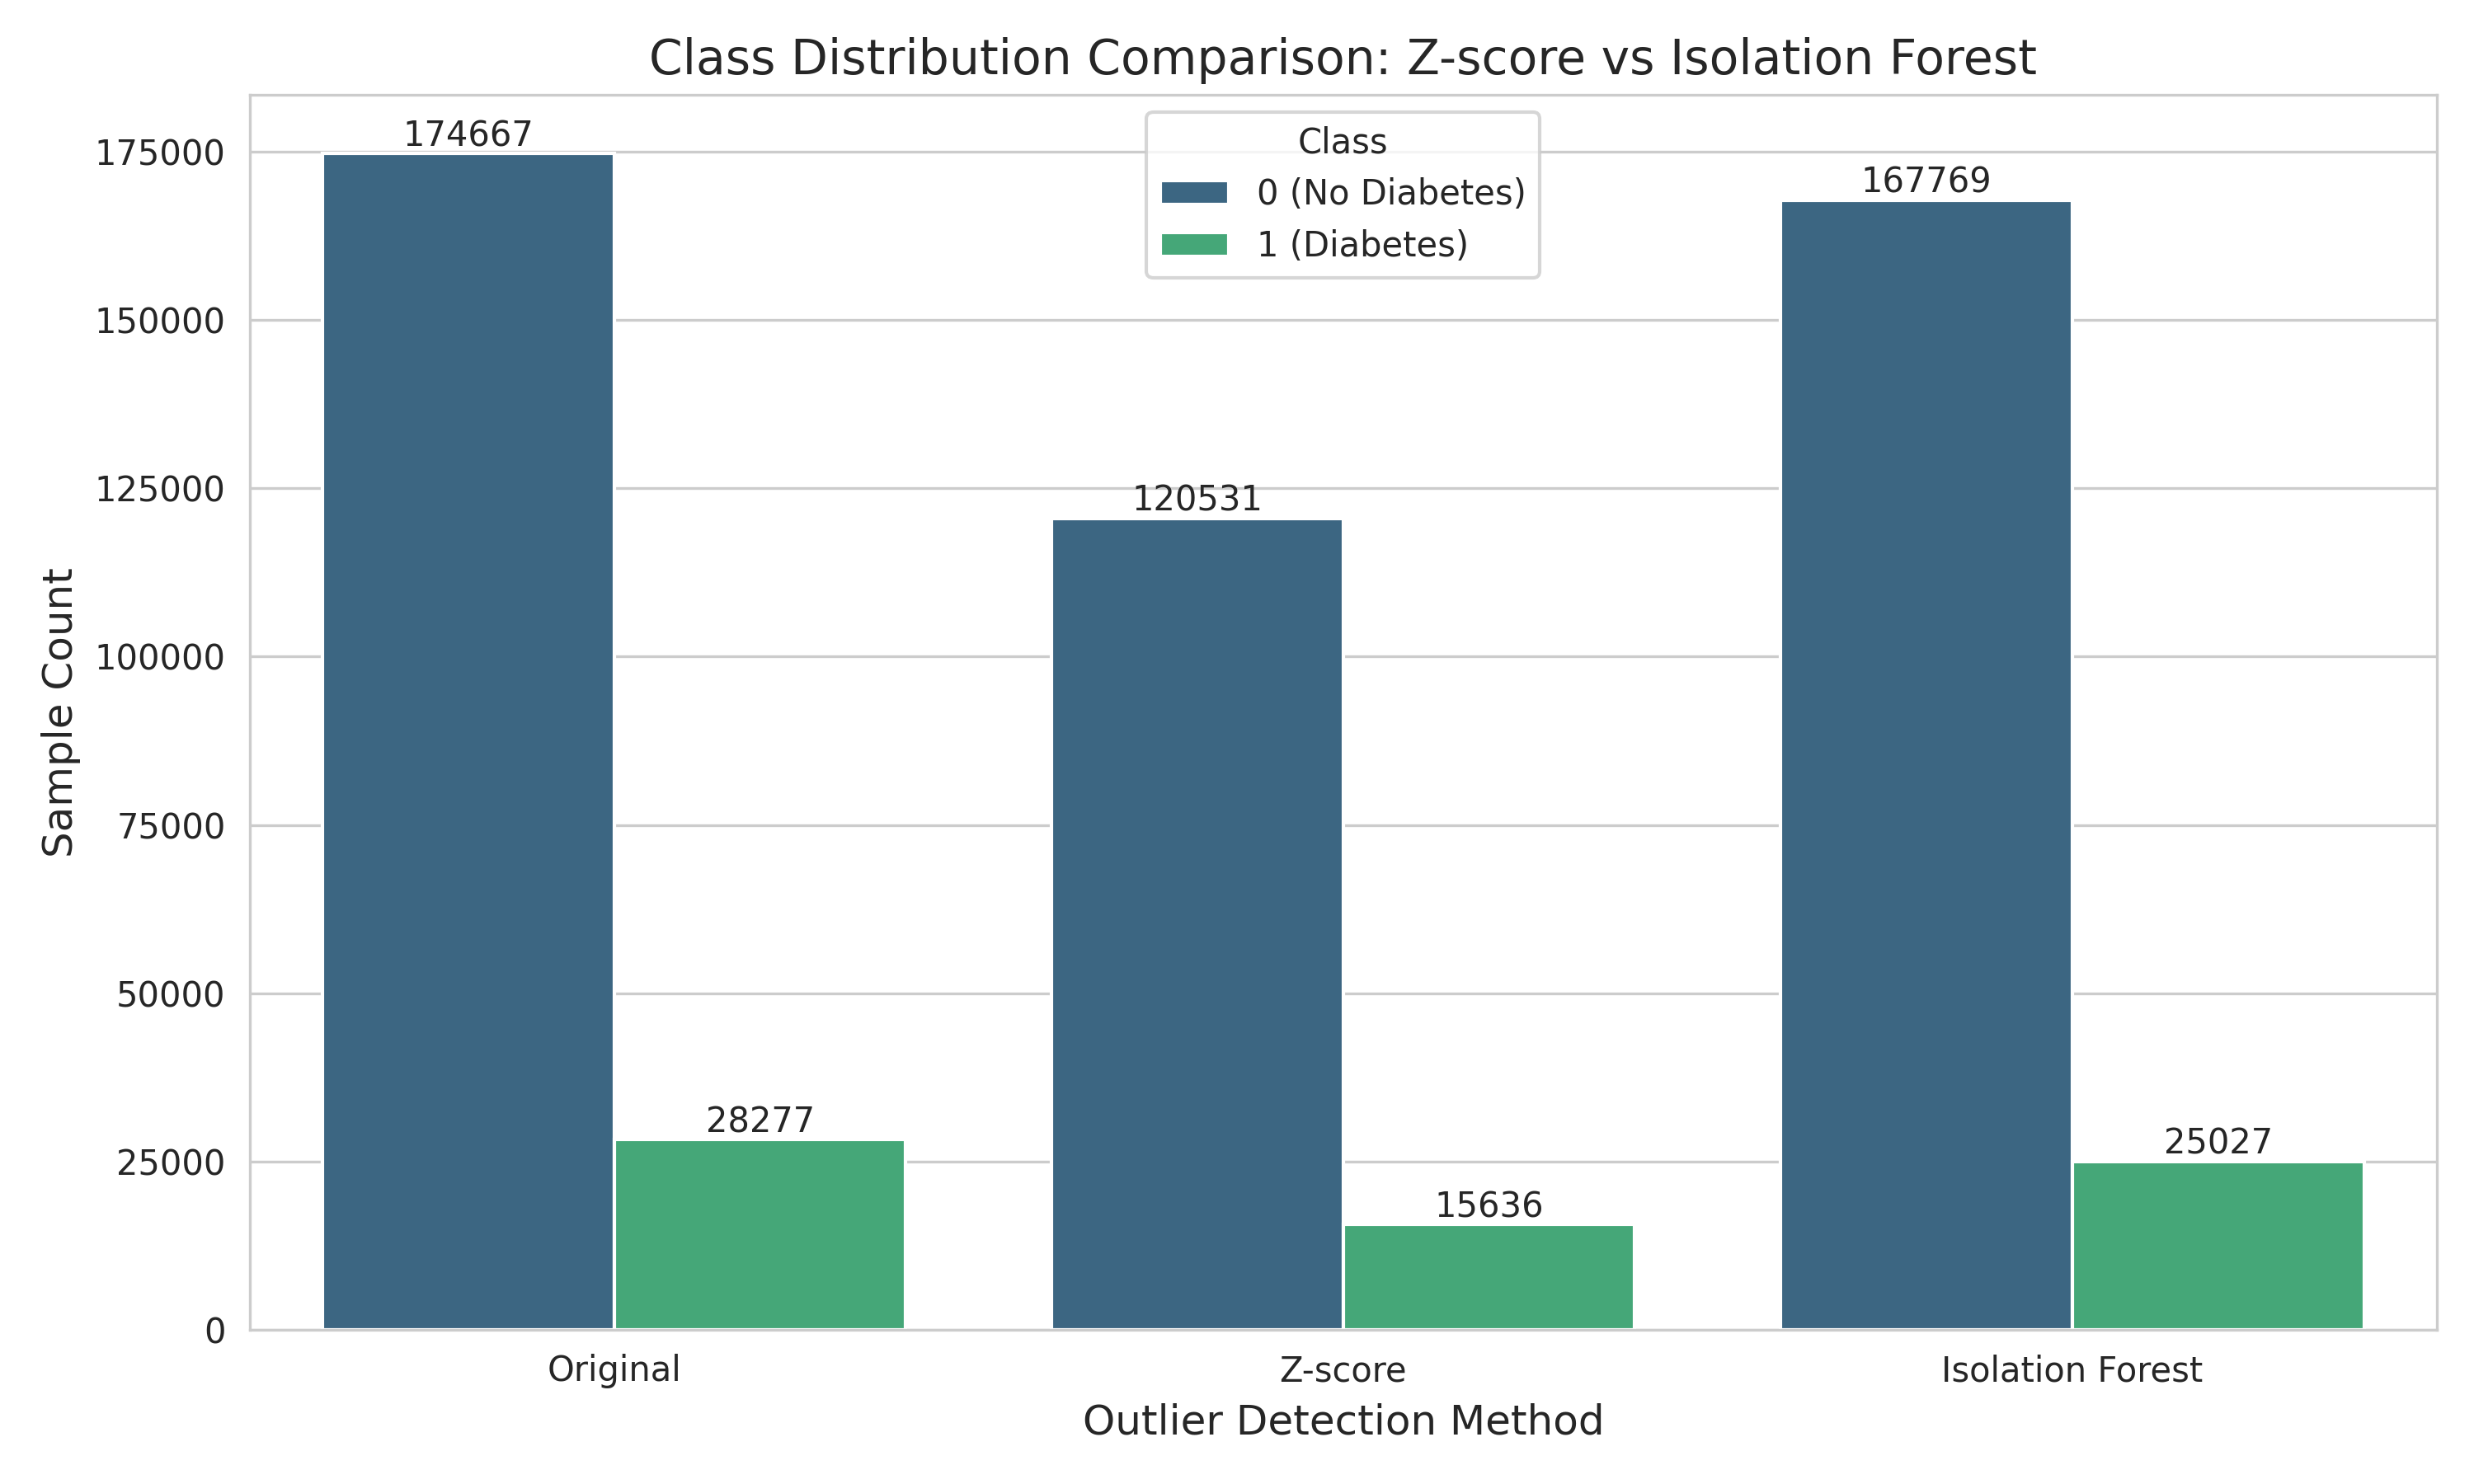
\includegraphics[width=0.9\linewidth]{figures/class_distribution_comparison.png}}
\caption{Class Distributions: Original vs. Z-score vs. Isolation Forest.}
\label{fig:class_dist}
\end{figure}

\begin{figure}[htbp]
\centerline{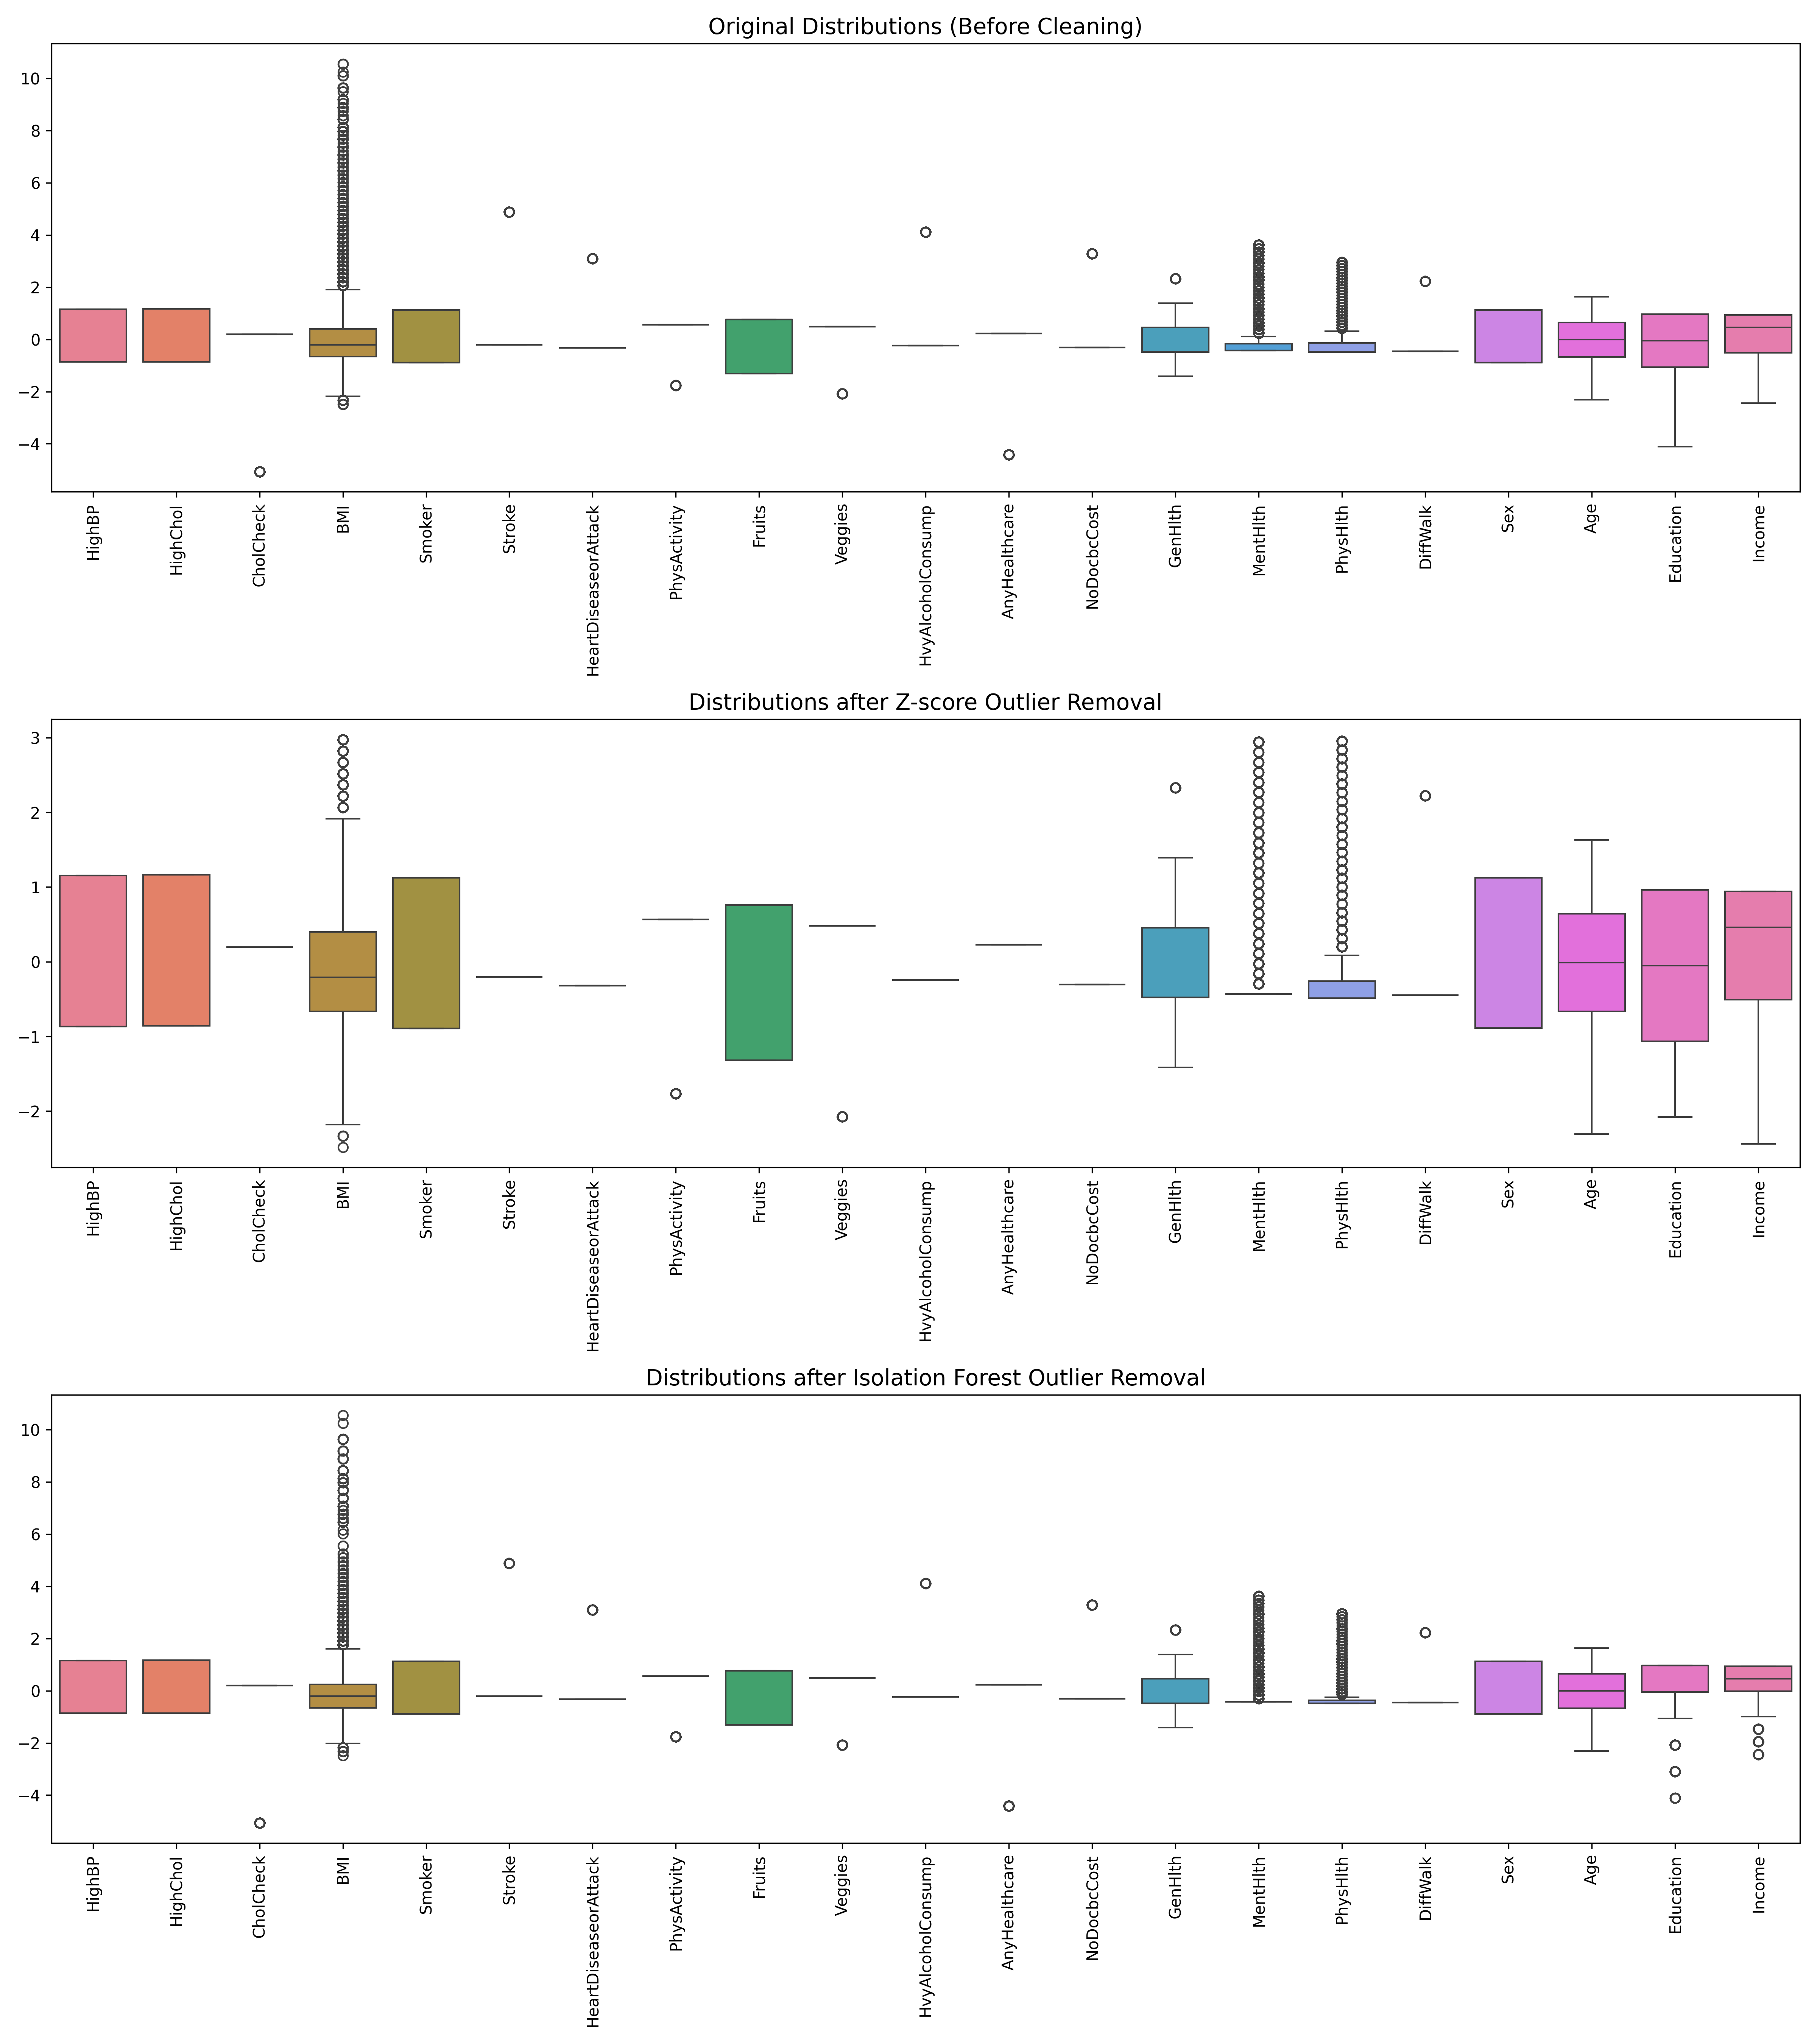
\includegraphics[width=1.0\linewidth]{figures/outlier_method_comparison.png}}
\caption{Feature distributions: Isolation Forest vs. Z-score.}
\label{fig:outlier_comp}
\end{figure}

Figures \ref{fig:pairplot}, \ref{fig:feature_hist}, and \ref{fig:corr_heatmap} highlight the complex, non-linear feature relationships.

\begin{figure}[htbp]
\centerline{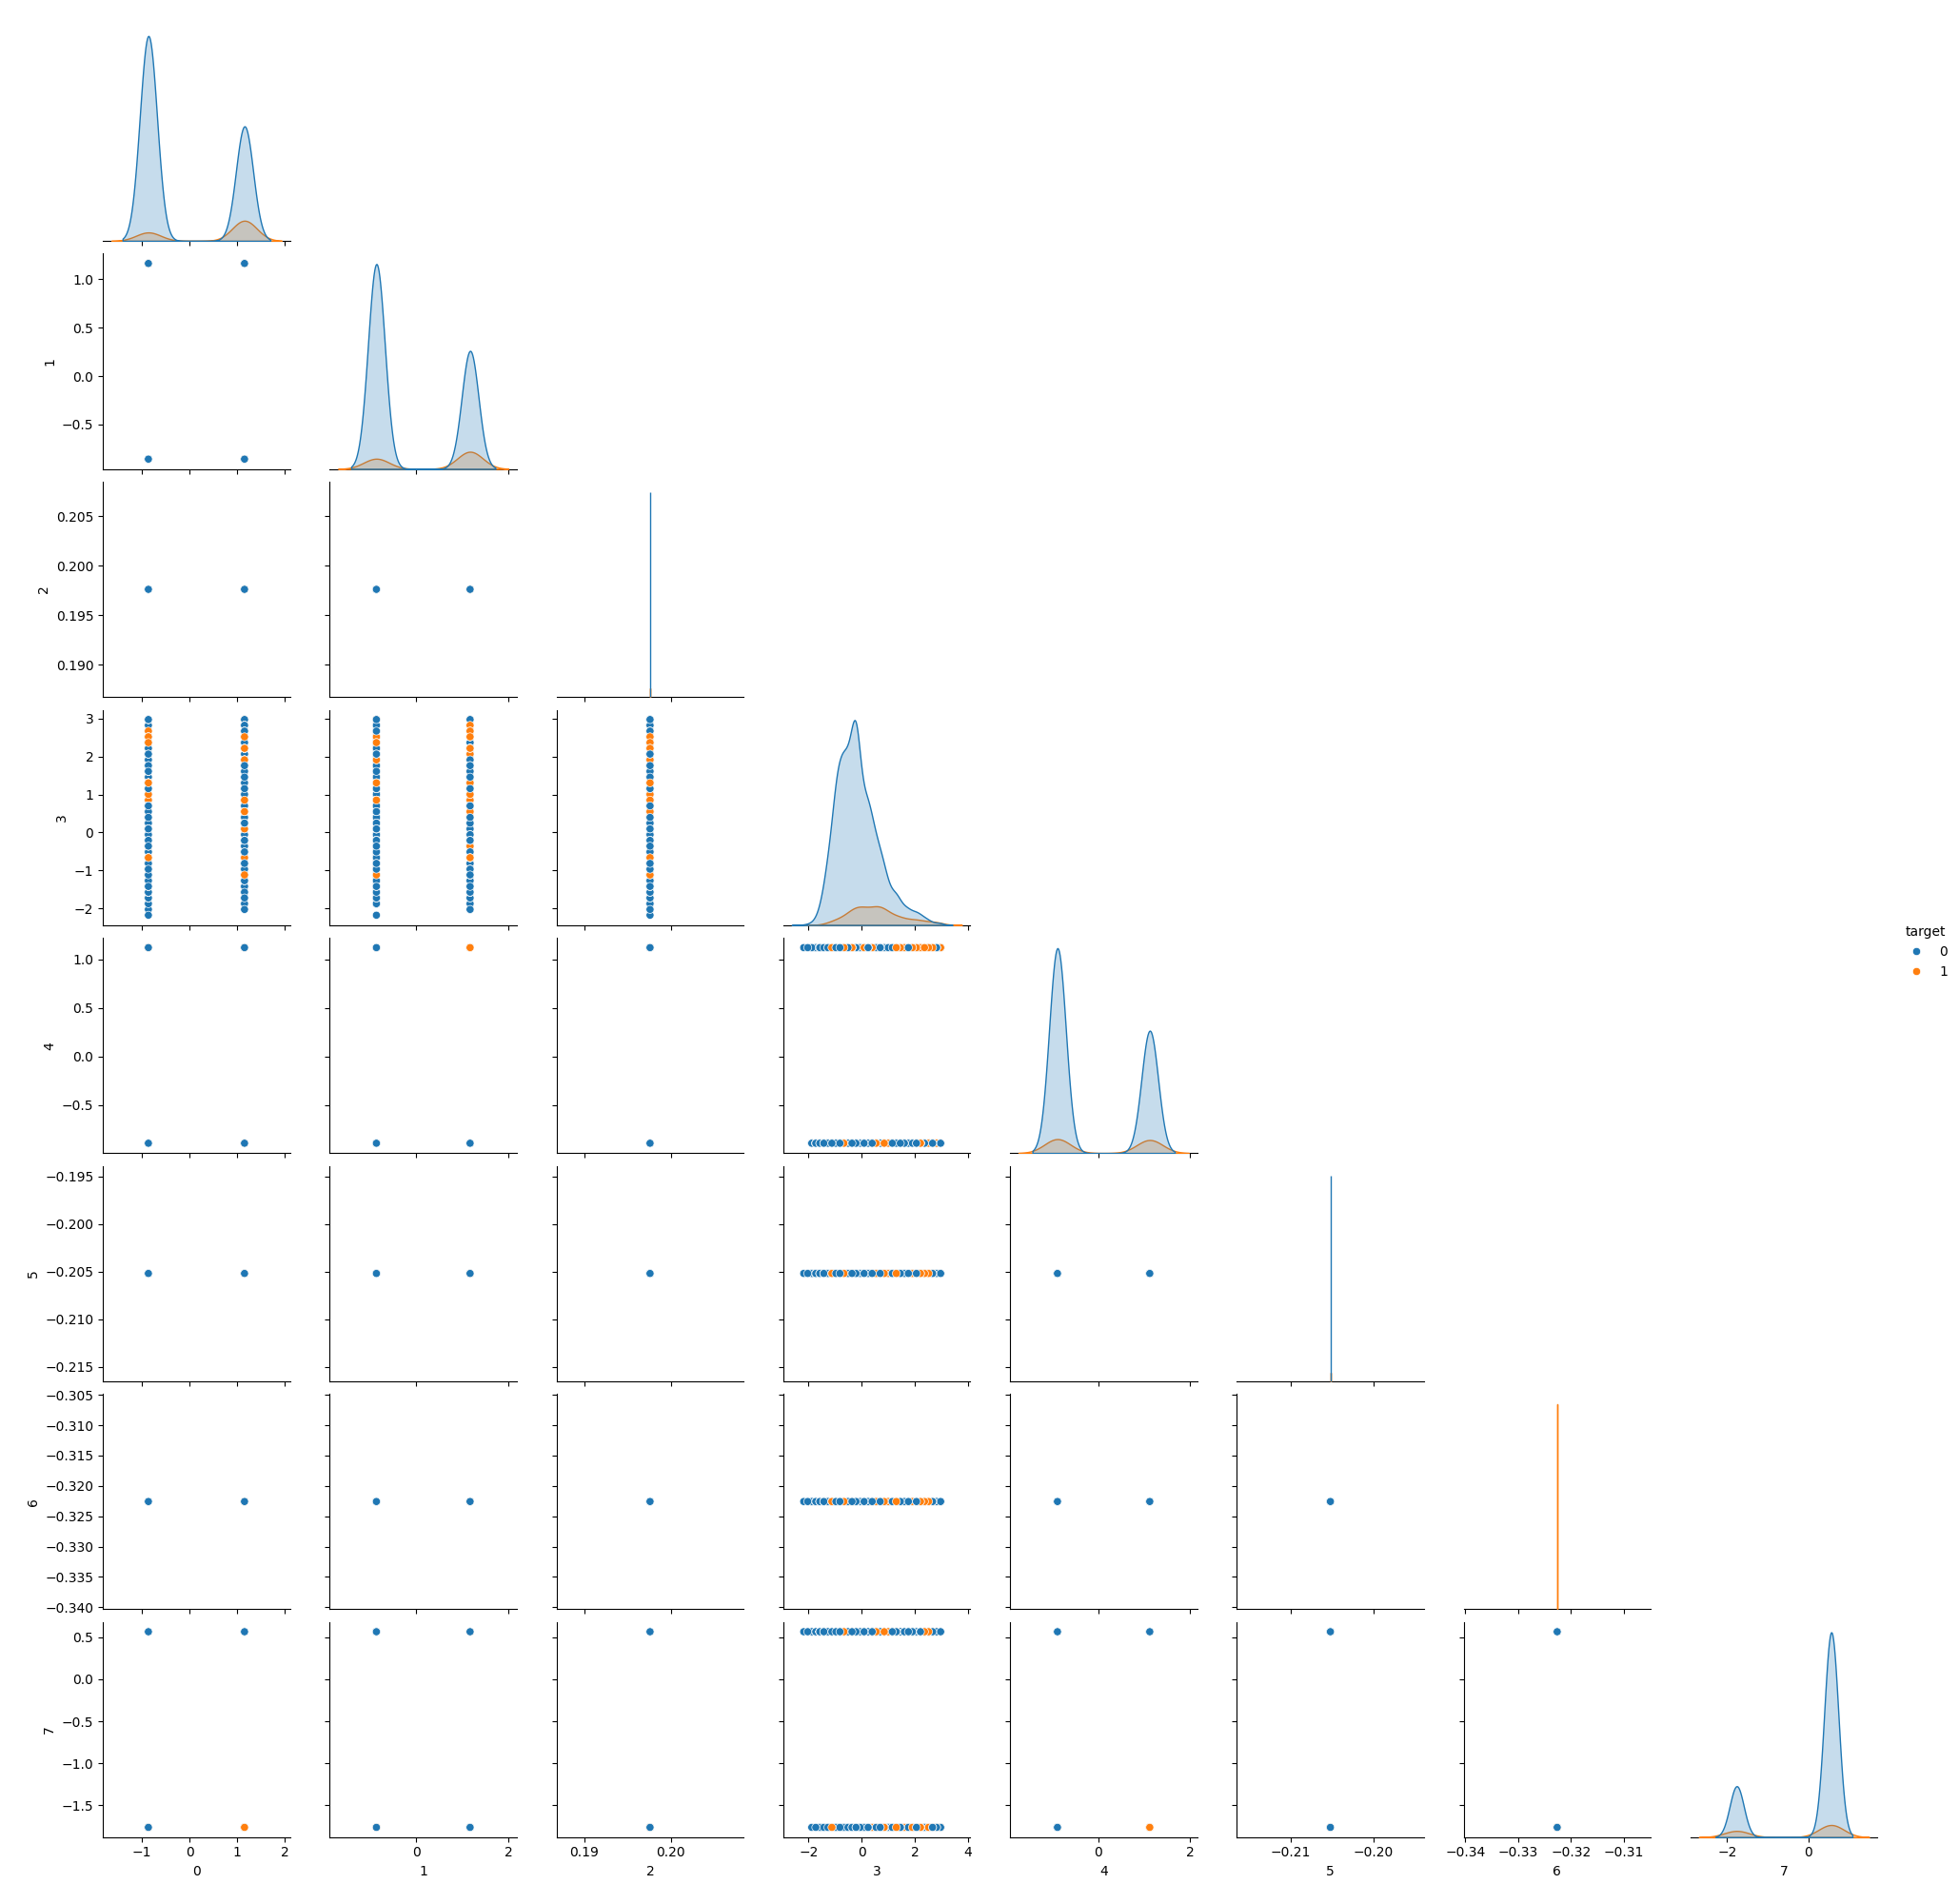
\includegraphics[width=0.9\linewidth]{figures/pairplot.png}}
\caption{Pairplot of selected features.}
\label{fig:pairplot}
\end{figure}

\begin{figure}[htbp]
\centering
\includegraphics[width=0.8\linewidth]{figures/feature_hist.png}
\caption{Feature distributions.}
\label{fig:feature_hist}
\end{figure}

\begin{figure}[htbp]
\centering
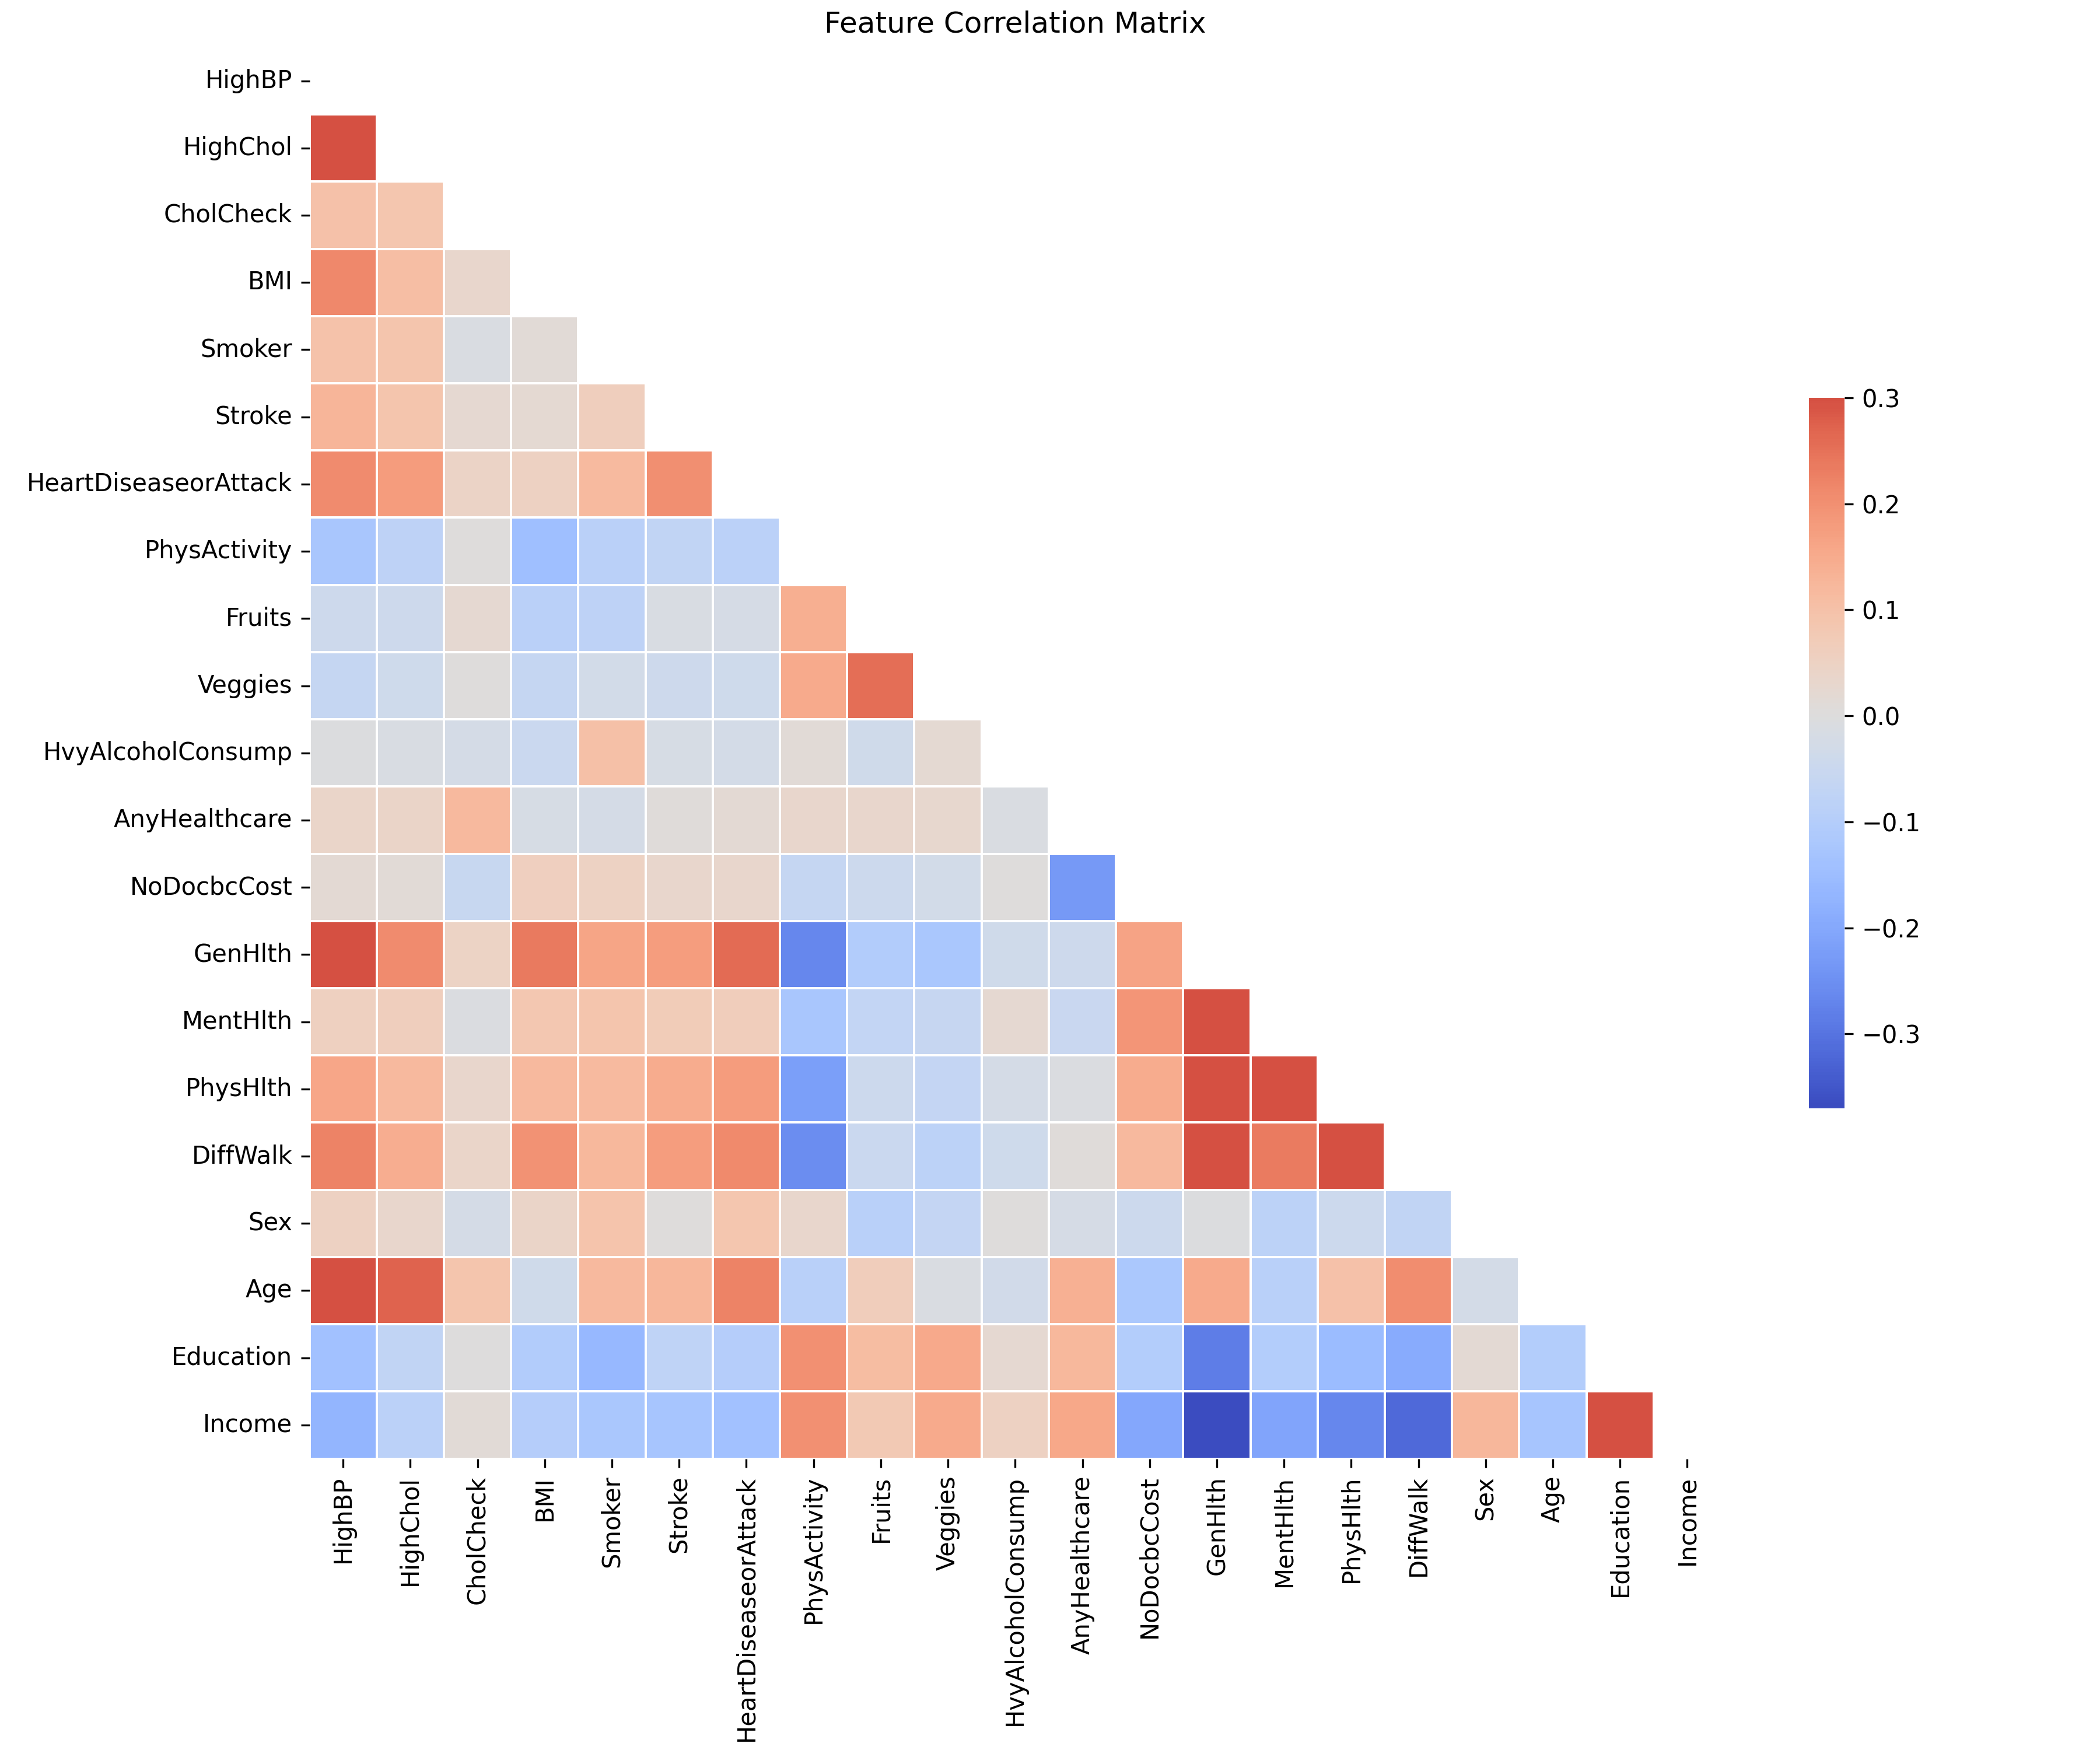
\includegraphics[width=0.8\linewidth]{figures/corr_heatmap.png}
\caption{Correlation heatmap.}
\label{fig:corr_heatmap}
\end{figure}

\subsection{Representation Learning}
We investigate three input formats: Raw features, **PCA** (linear projection), and **Autoencoder (AE)** embeddings (non-linear compression). PCA visualizations (Figs. \ref{fig:pca_labels}-\ref{fig:pca_clusters_iso}) reveal significant class overlap. UMAP (Fig. \ref{fig:umap_comp}) confirms Isolation Forest preserves manifold structure better than Z-score.

\begin{figure}[htbp]
\centerline{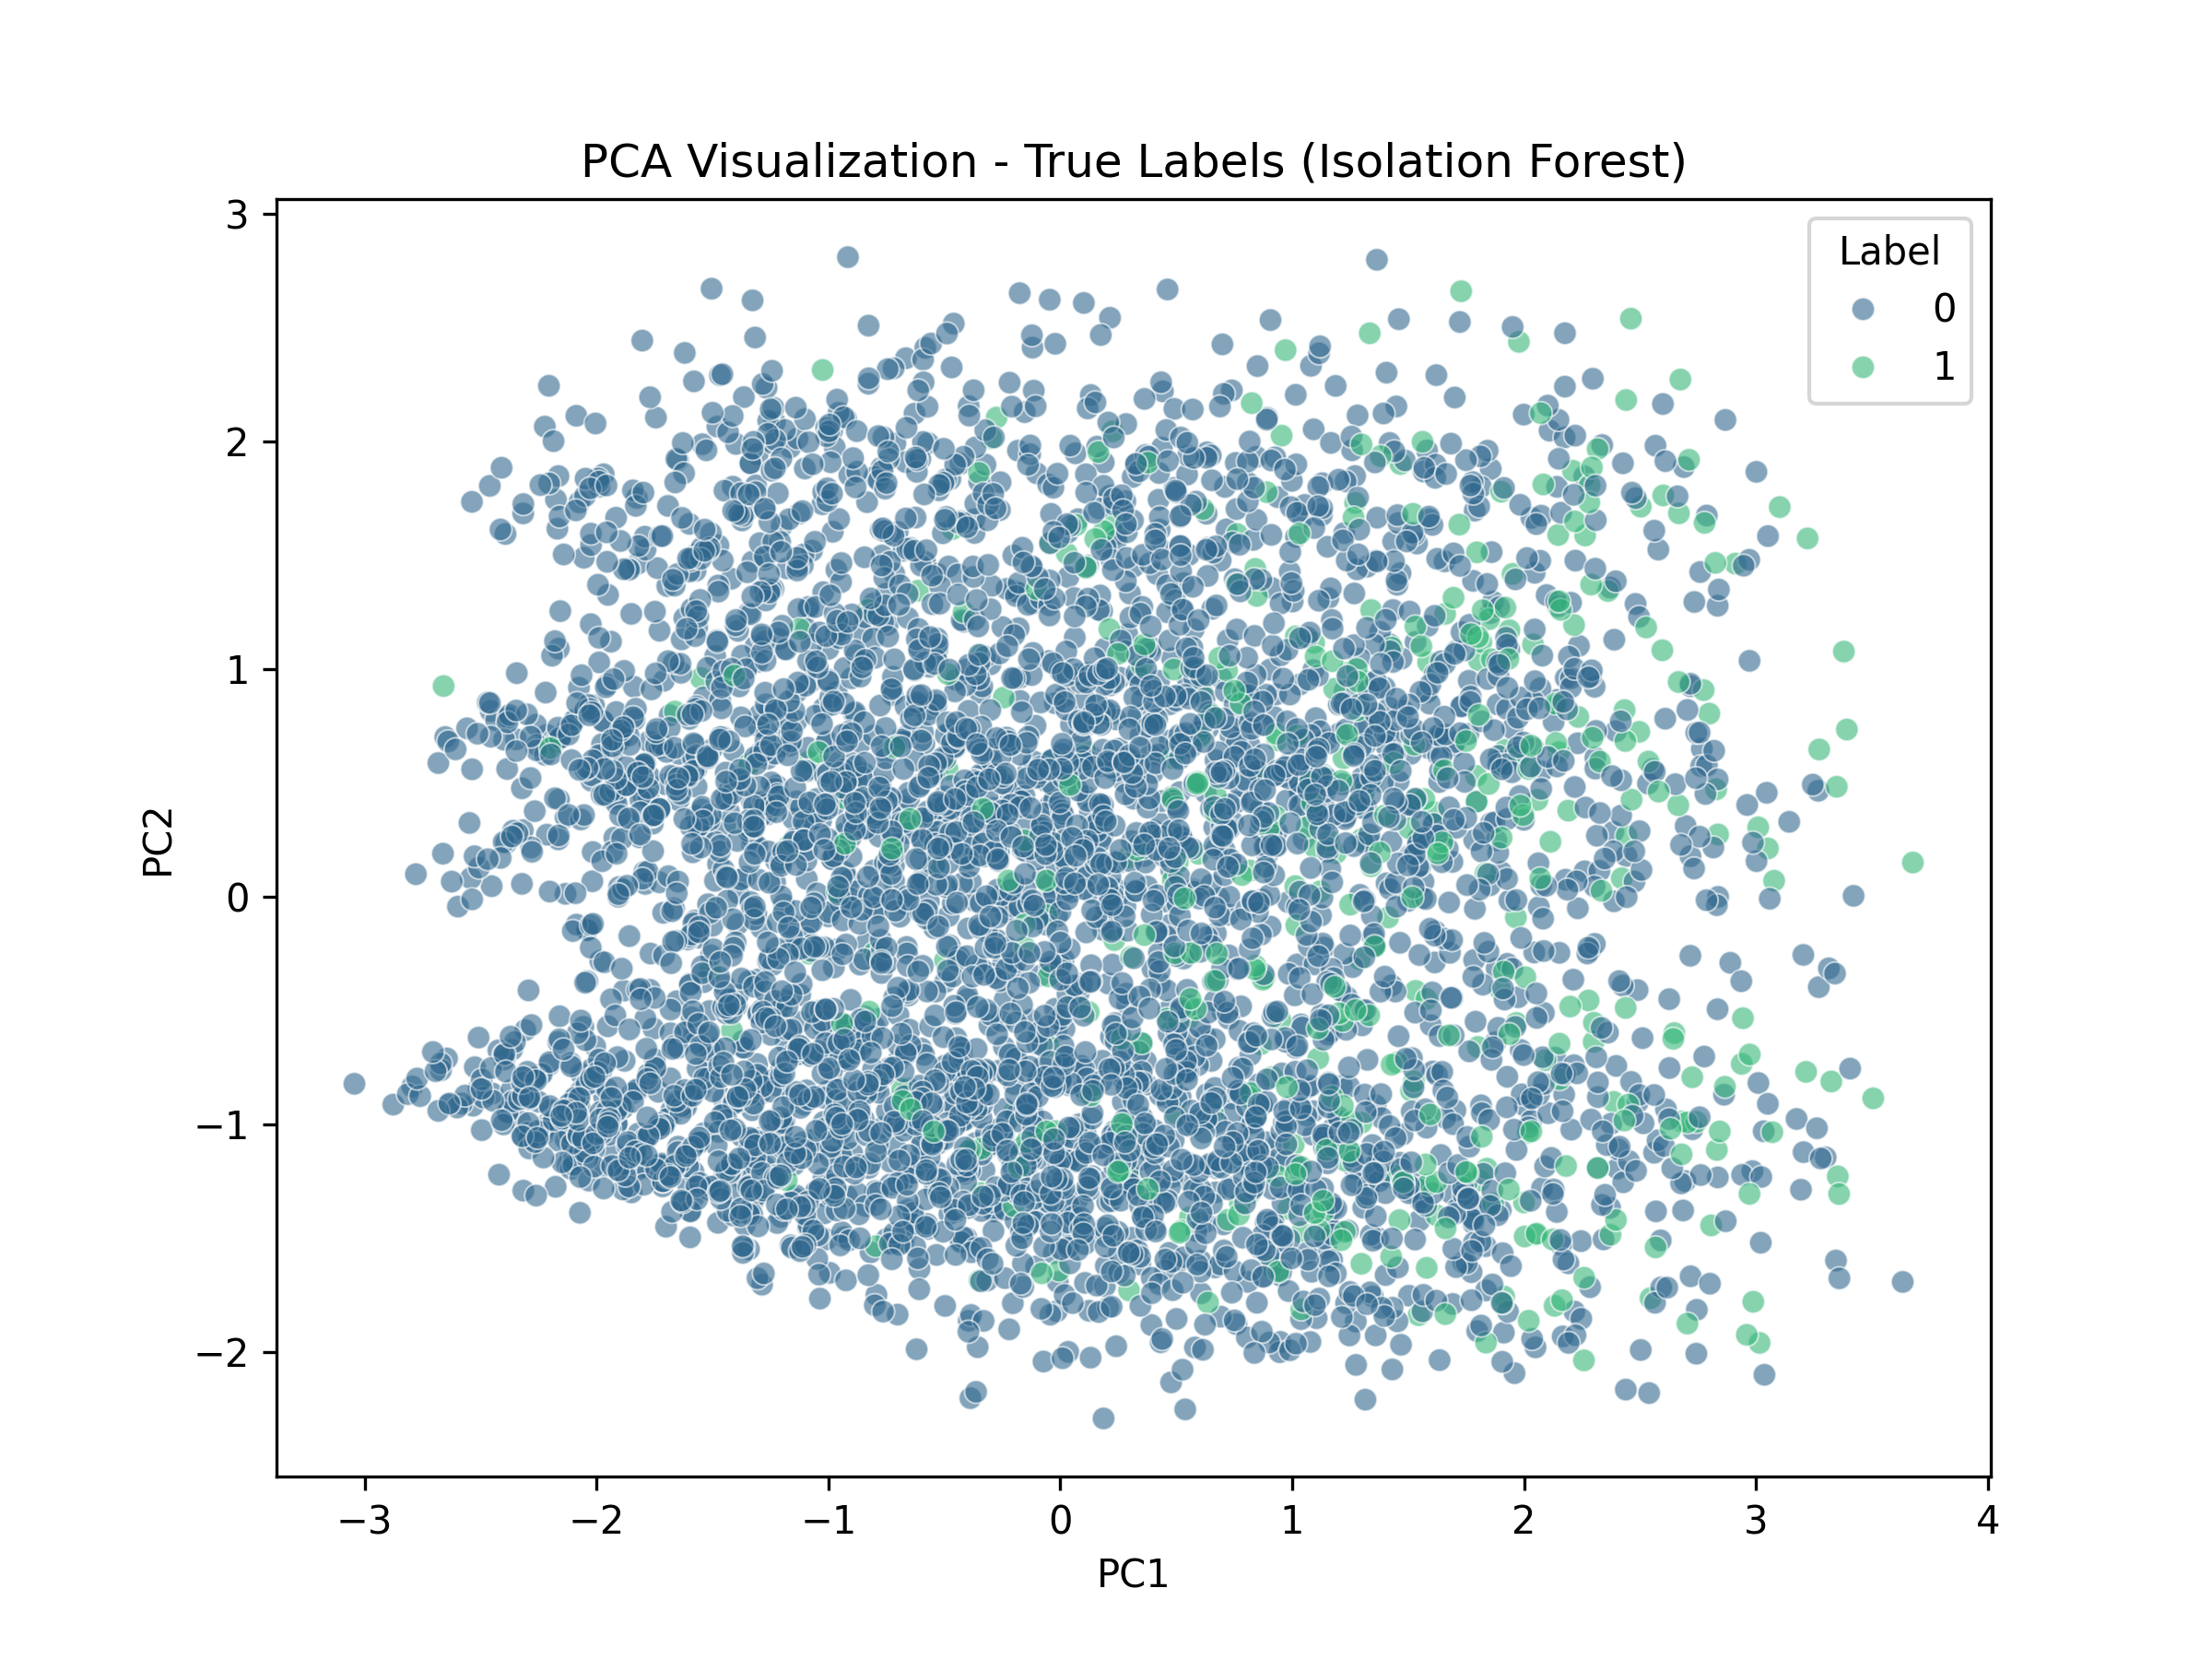
\includegraphics[width=0.9\linewidth]{figures/unsupervised_pca_labels_iso.png}}
\caption{PCA Visualization (Isolation Forest).}
\label{fig:pca_labels_iso}
\end{figure}

\begin{figure}[htbp]
\centerline{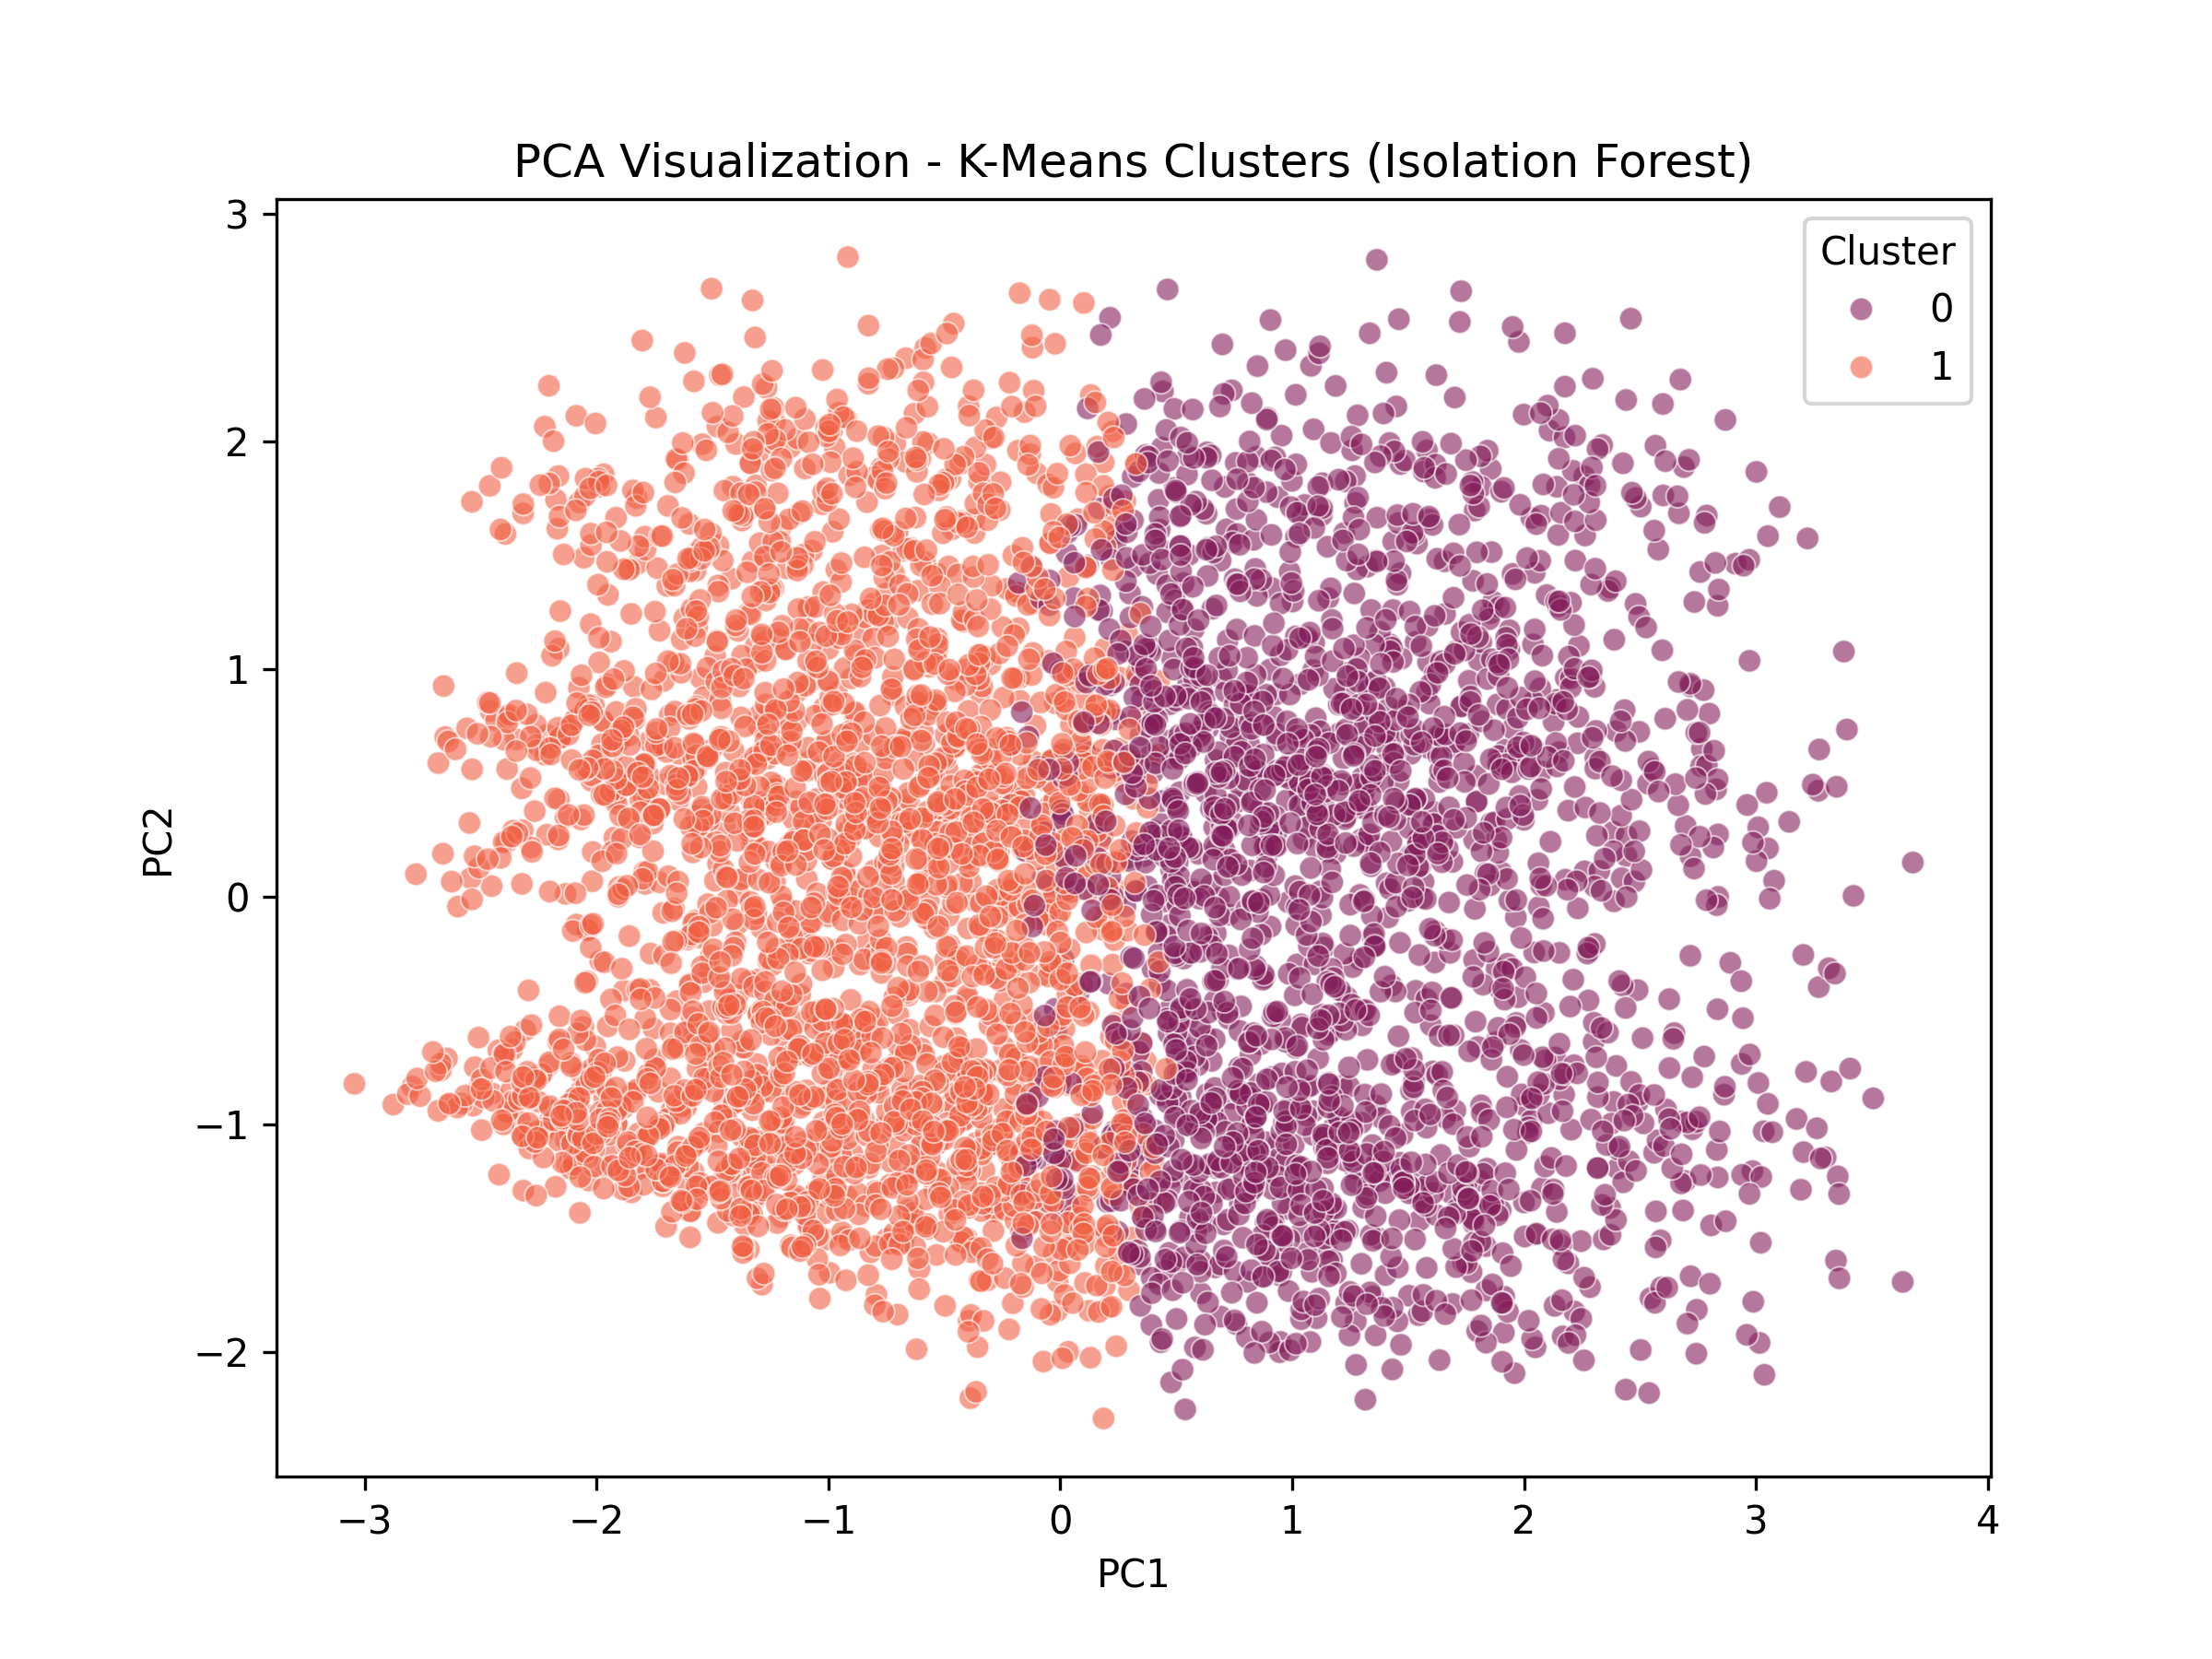
\includegraphics[width=0.9\linewidth]{figures/unsupervised_pca_clusters_iso.png}}
\caption{PCA K-Means Clusters.}
\label{fig:pca_clusters_iso}
\end{figure}

\begin{figure}[htbp]
\centerline{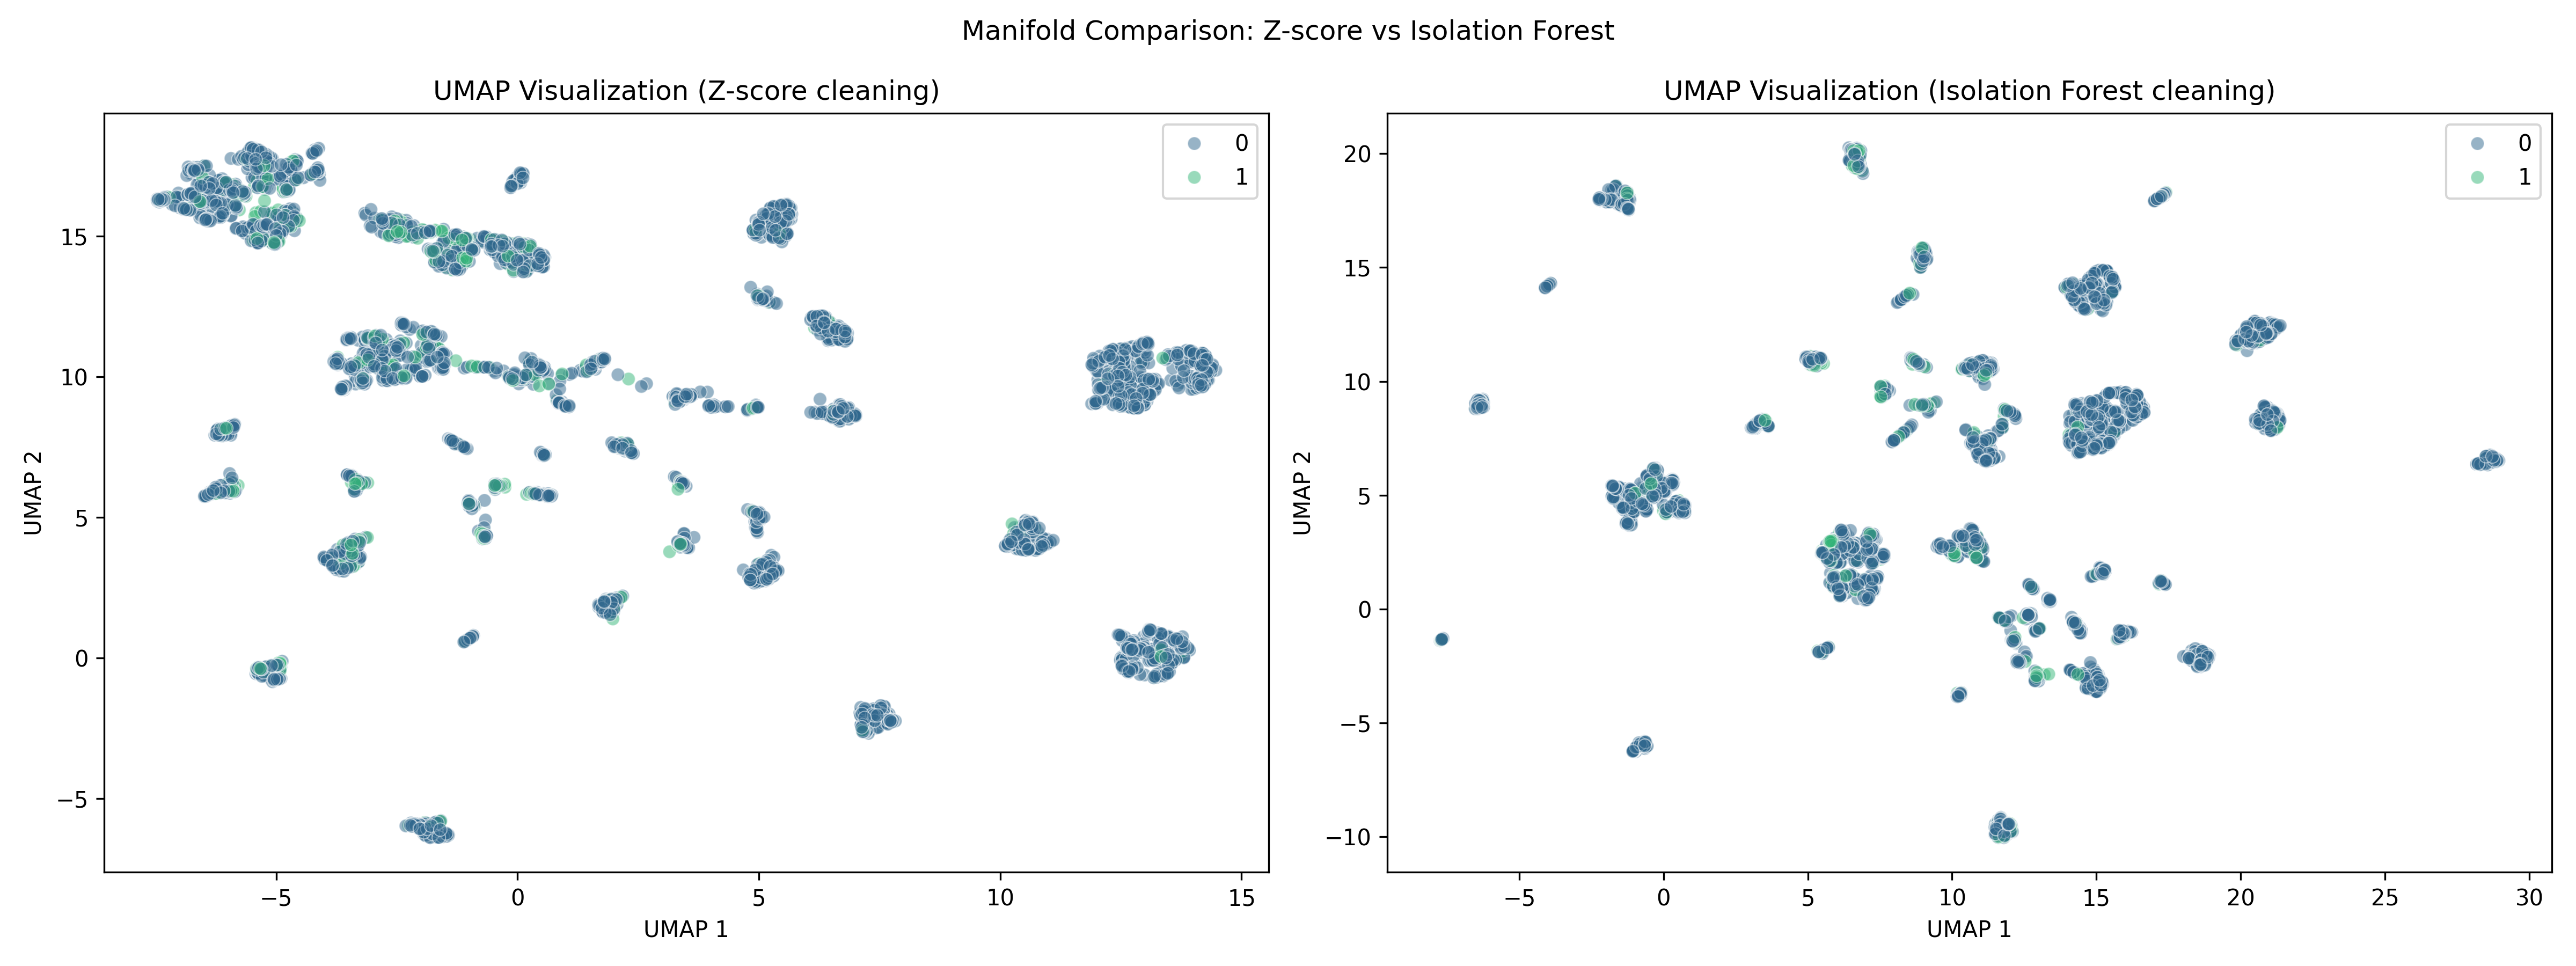
\includegraphics[width=1.0\linewidth]{figures/umap_comparison.png}}
\caption{UMAP: Z-score vs. Isolation Forest.}
\label{fig:umap_comp}
\end{figure}

The AE minimizes reconstruction loss $\mathcal{L}_{AE} = ||\bx - g_\phi(f_\theta(\bx))||^2 + \lambda ||\theta||^2$ to capture latent features (Figs. \ref{fig:ae_arch}-\ref{fig:ae_latent_iso}).

\begin{figure}[htbp]
\centerline{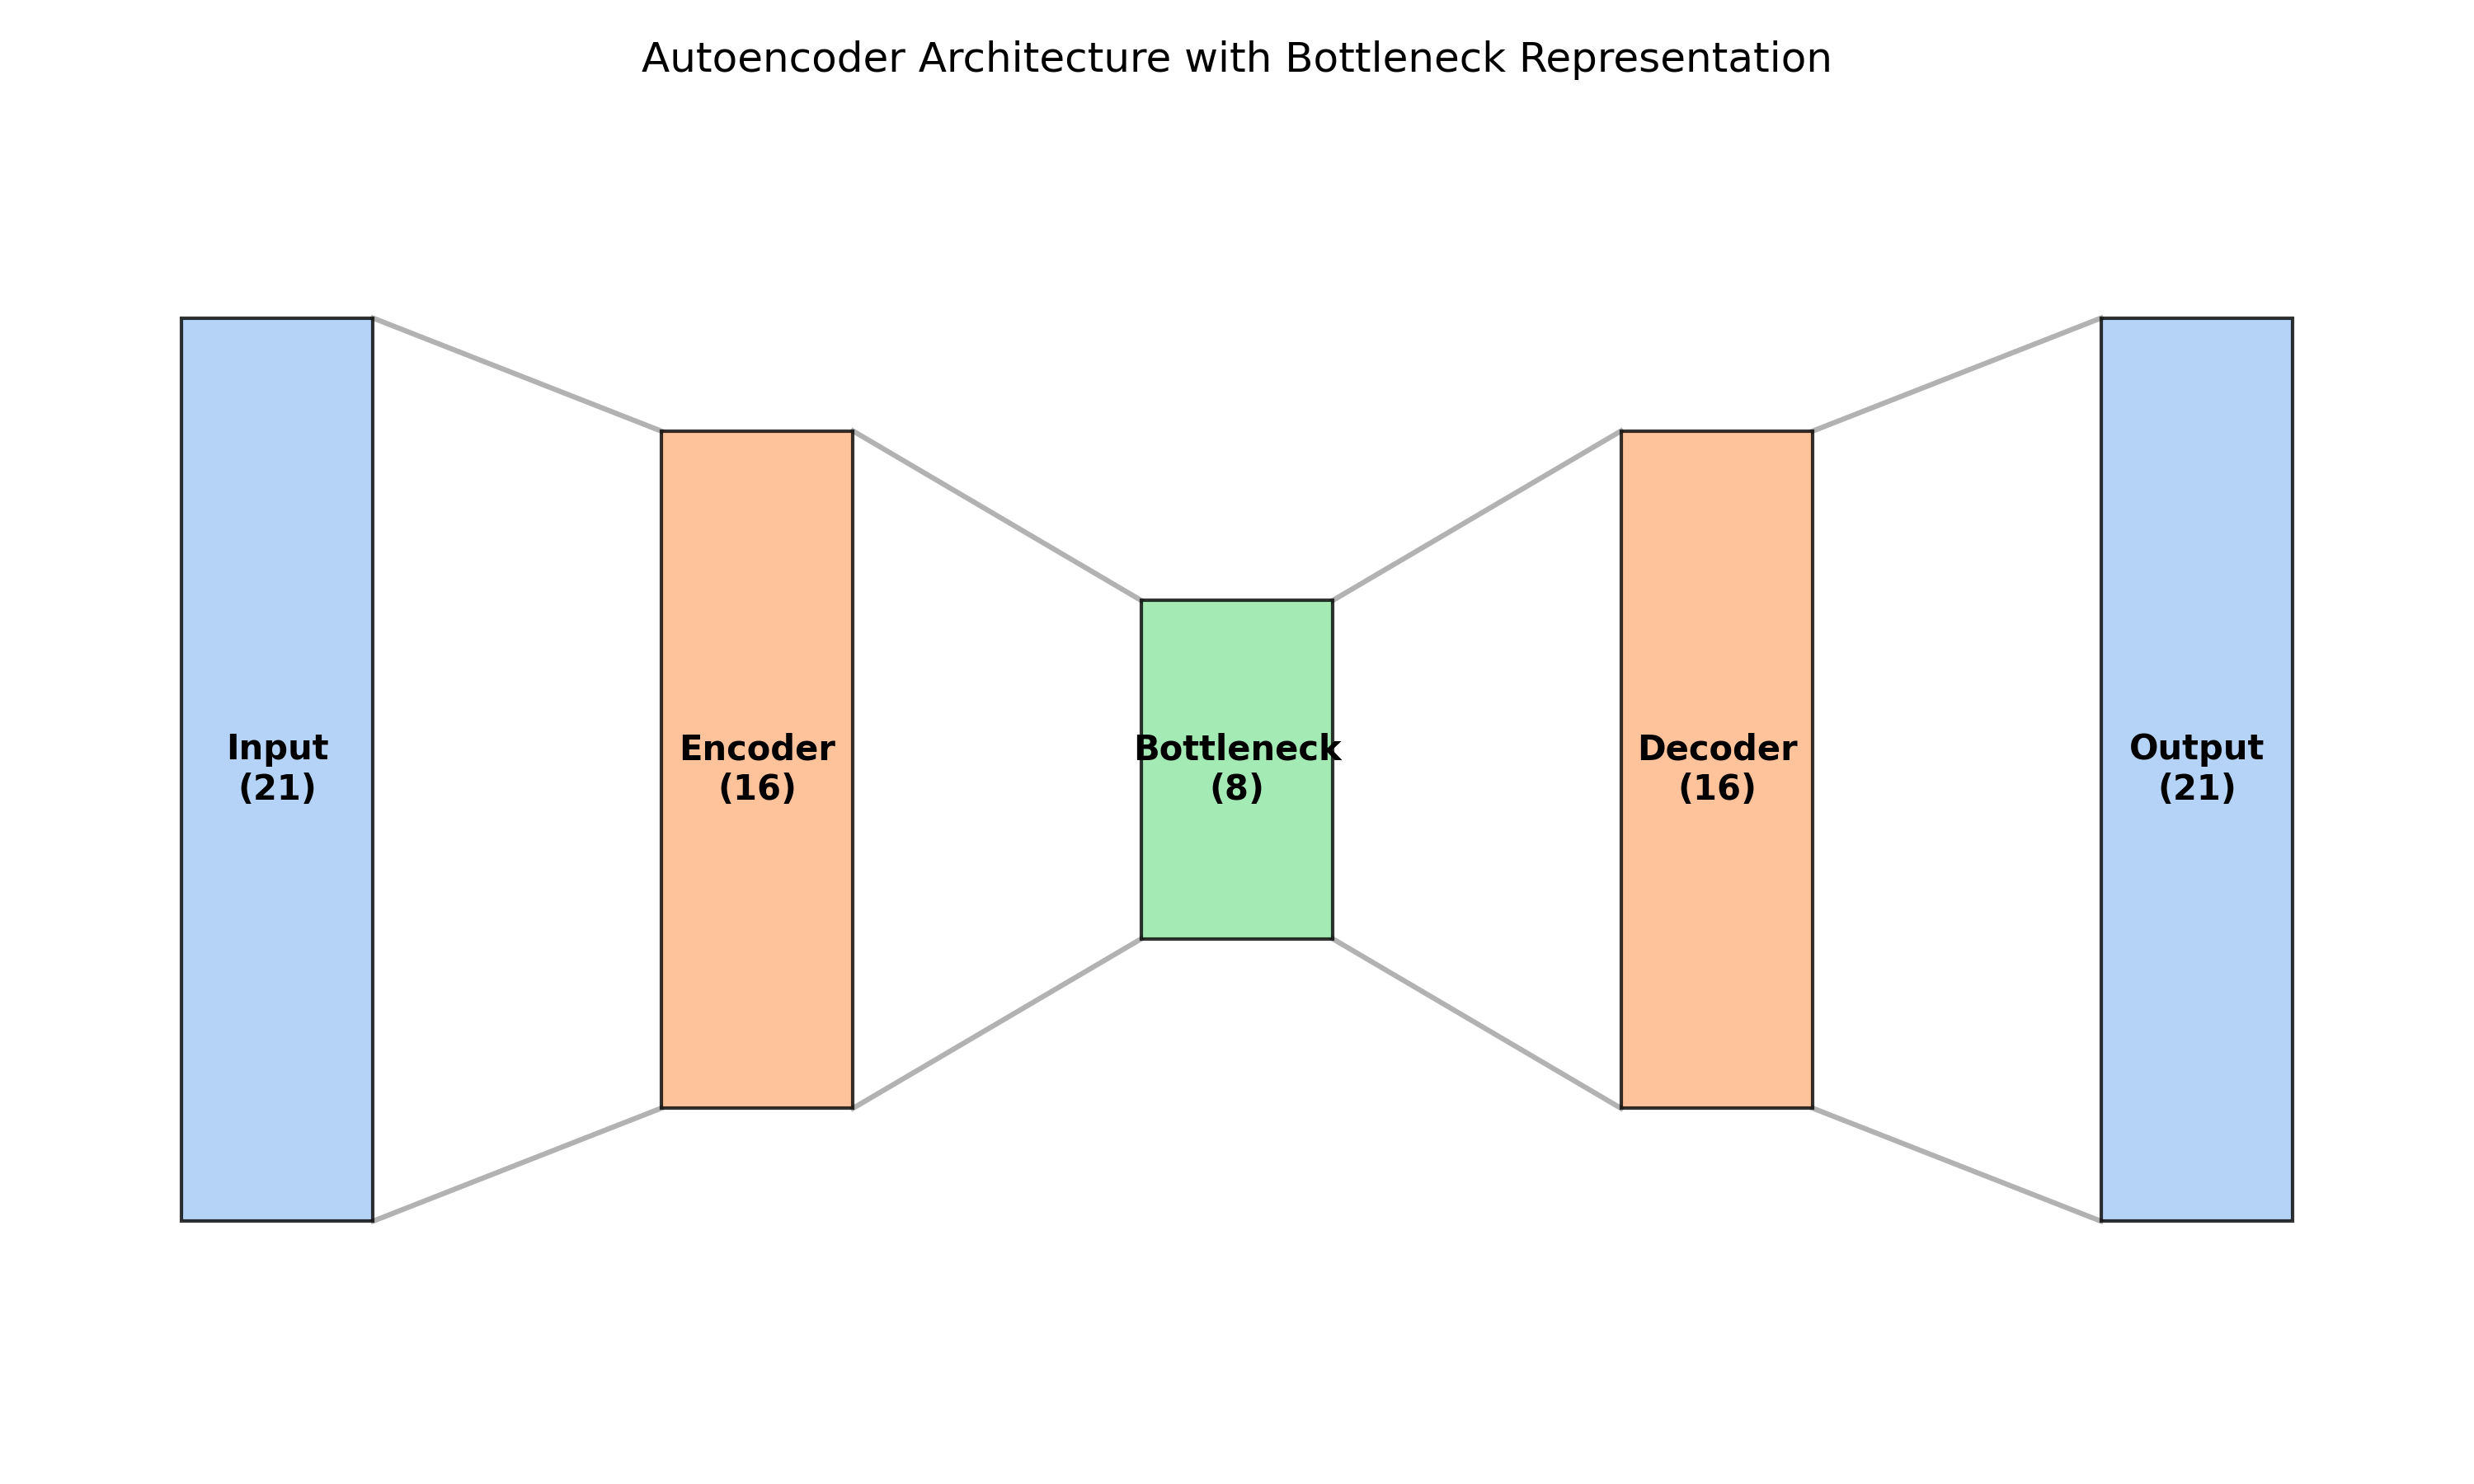
\includegraphics[width=0.9\linewidth]{figures/autoencoder_arch.png}}
\caption{Autoencoder Architecture.}
\label{fig:ae_arch}
\end{figure}

\begin{figure}[htbp]
\centerline{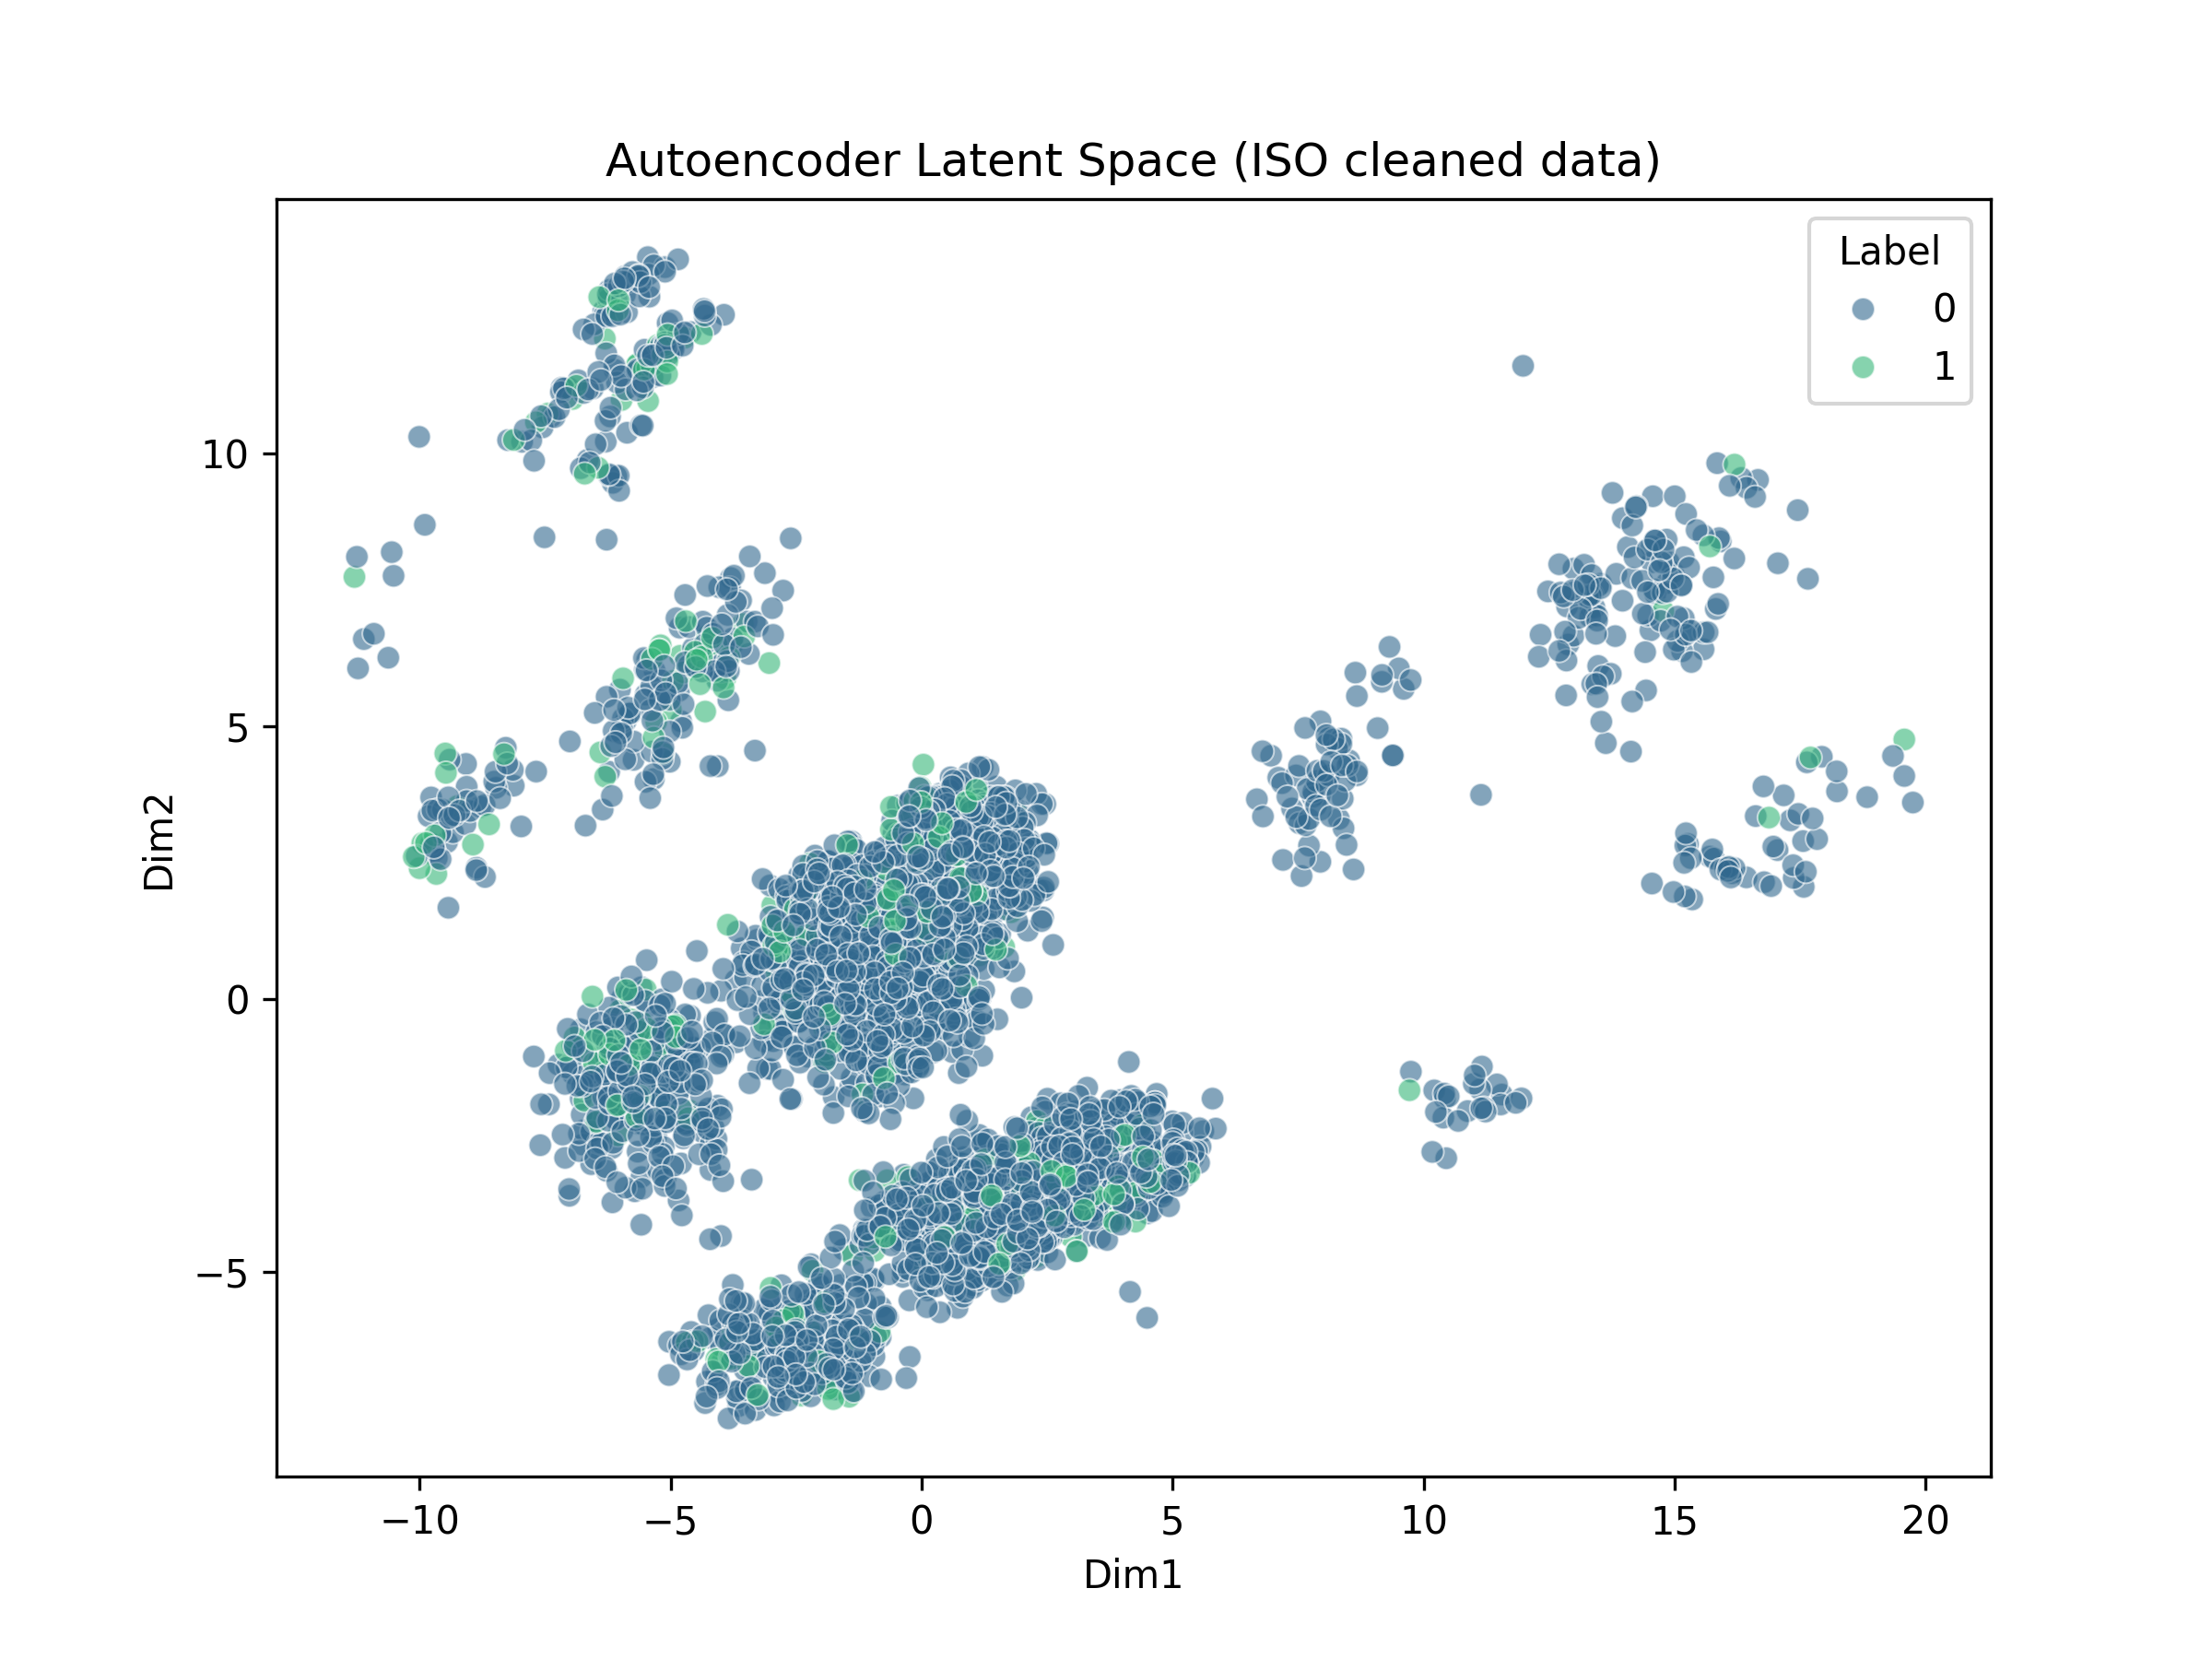
\includegraphics[width=0.9\linewidth]{figures/unsupervised_ae_labels_iso.png}}
\caption{AE Latent Space (Isolation Forest).}
\label{fig:ae_latent_iso}
\end{figure}

\subsection{Baseline Neural Network & HPO}
We employ a fixed MLP (Fig. \ref{fig:mlp_arch}) with two dense layers (32, 16 neurons, ReLU) and a sigmoid output. We optimized hyperparameters (Learning Rate, Batch Size, Decay, Dropout) using:
*   **Random Search:** Stochastic baseline.
*   **Optuna:** Bayesian Optimization (TPE).
*   **Evolutionary Algorithms:** GA, DE, PSO, and Enhanced ALSHADE \cite{karpinski2025deullm}.

\begin{figure}[htbp]
\centerline{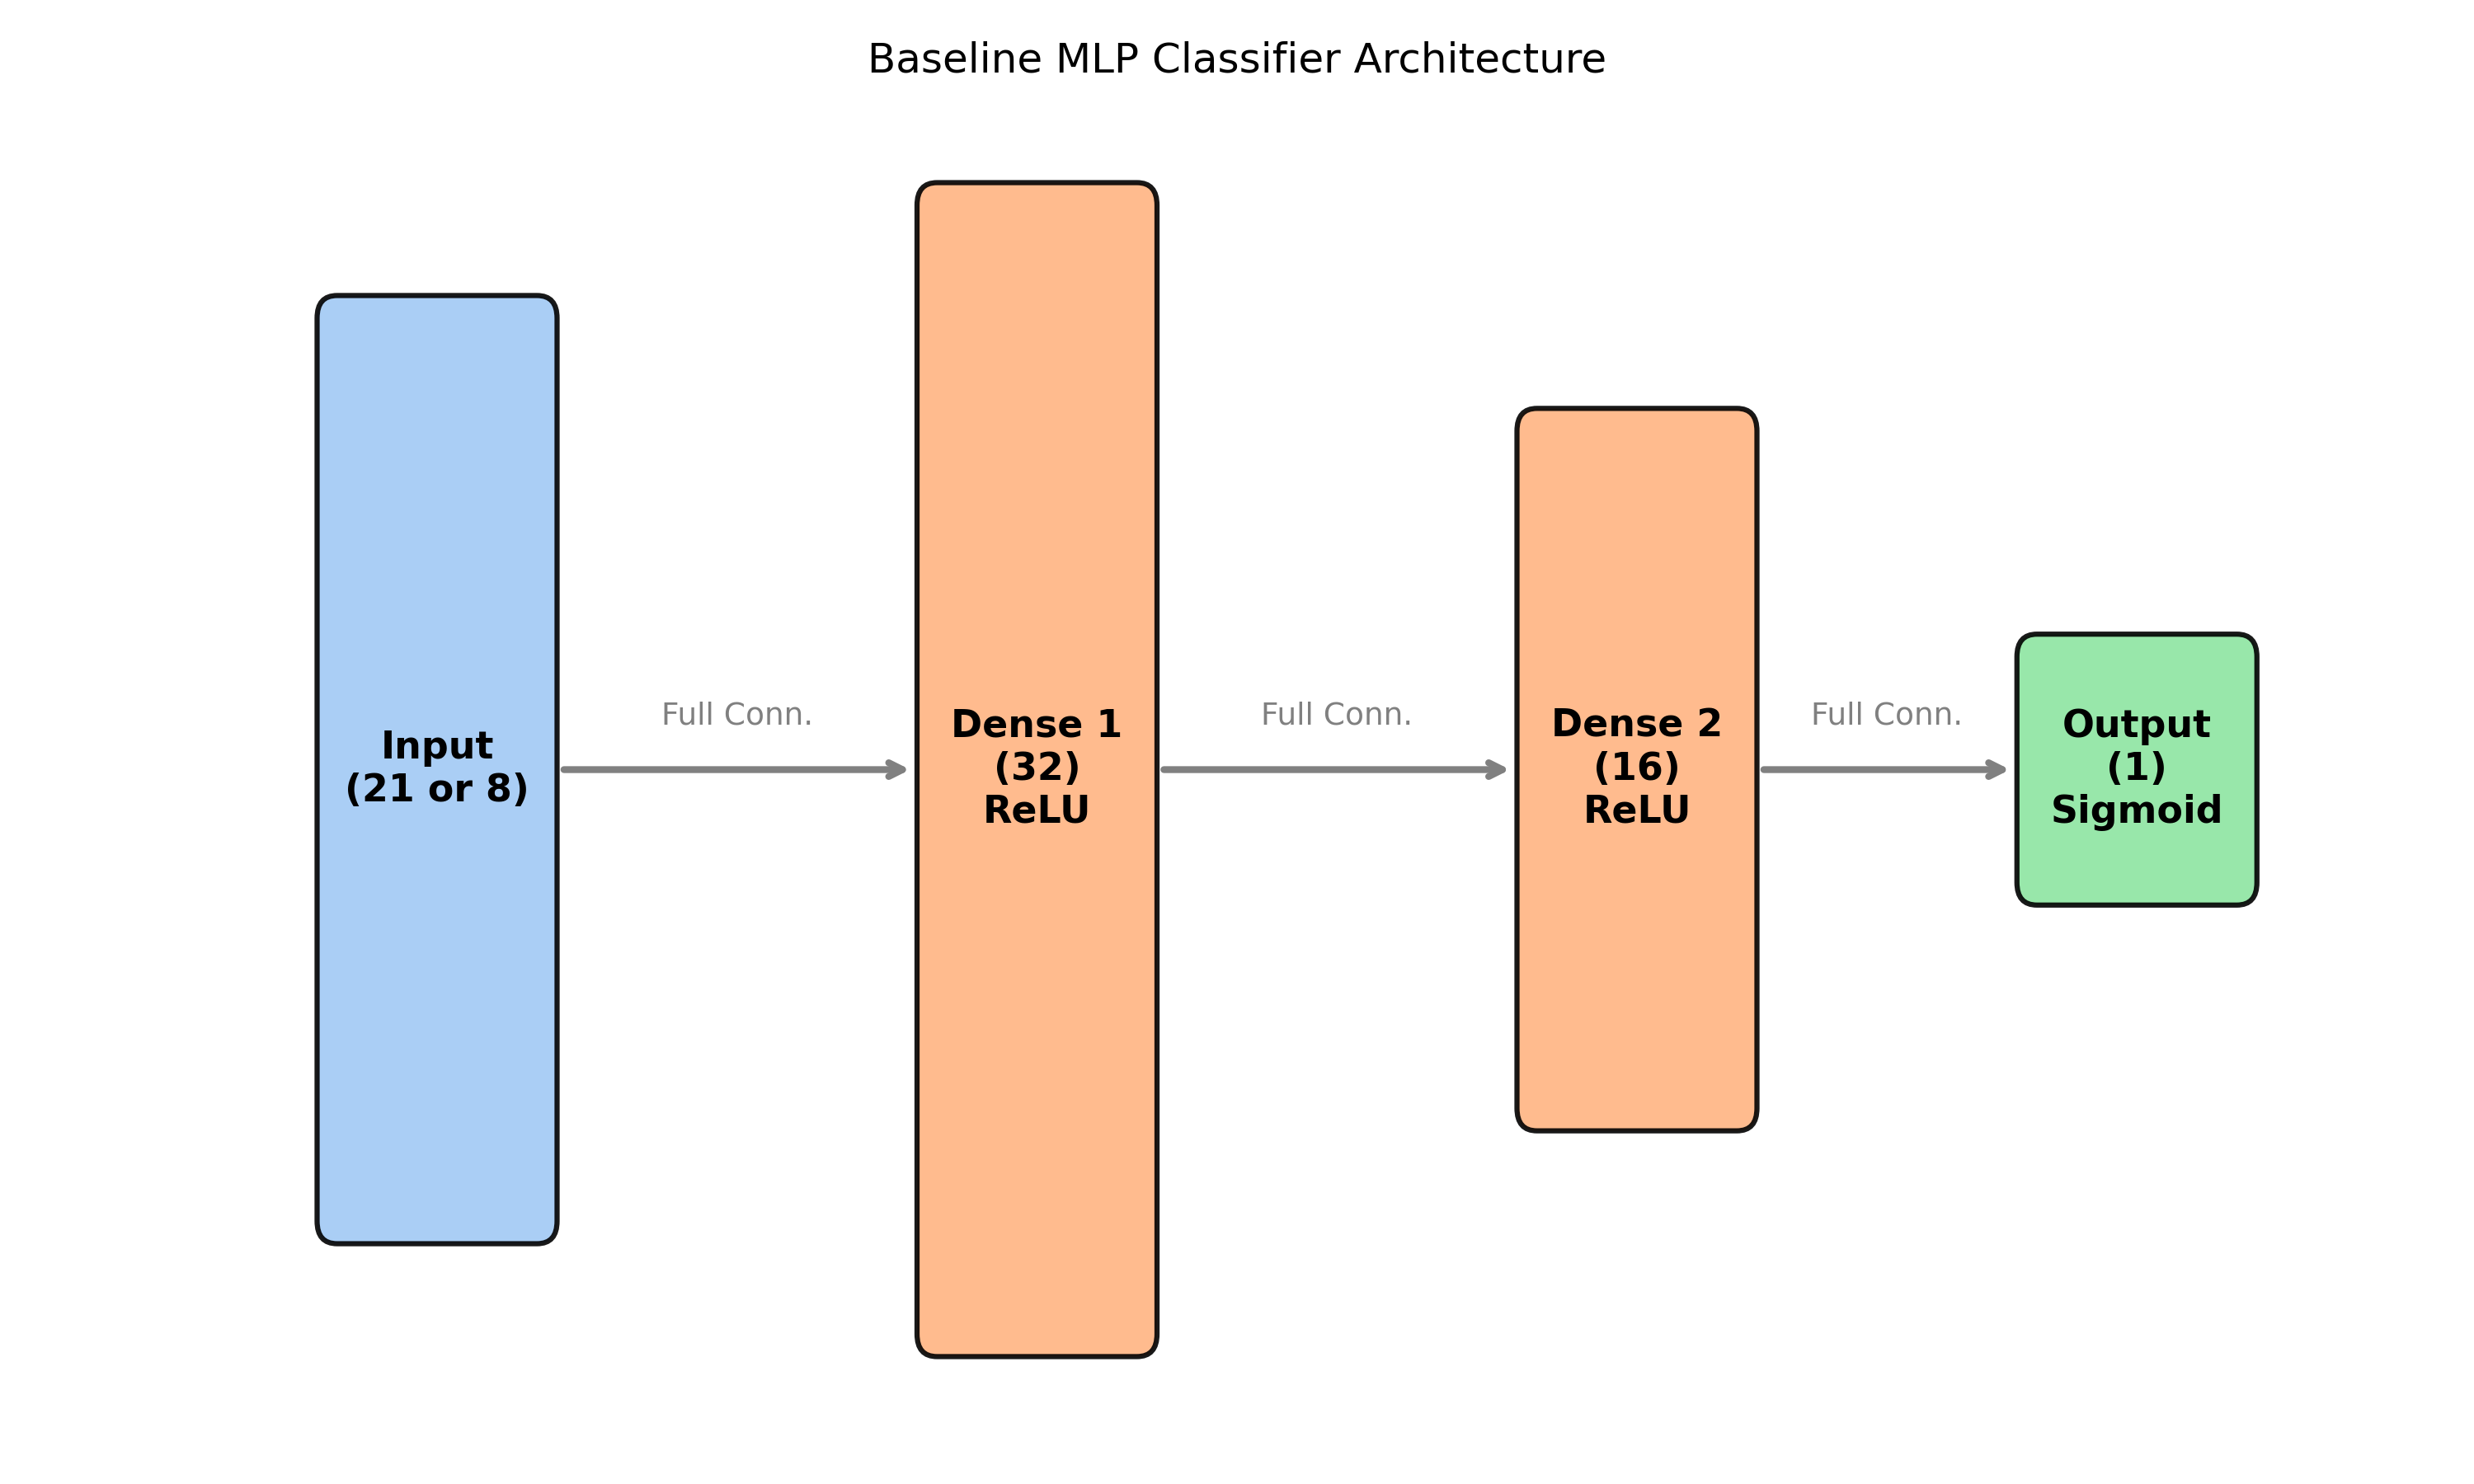
\includegraphics[width=0.9\linewidth]{figures/mlp_architecture.png}}
\caption{Baseline MLP Architecture.}
\label{fig:mlp_arch}
\end{figure}

\subsection{Neuro-Symbolic Interpretability Layer}
To audit the MLP, we implement a parallel expert layer:
1.  **Rule-Based:** Explicit heuristics (e.g., $BMI \ge 30 \land Age \ge 45 \rightarrow$ Risk).
2.  **Fuzzy Logic:** Models continuous variables (Age, BMI) into "Low/Medium/High" risk scores.
3.  **Bayesian Update:** A Gaussian Naive Bayes (GNB) classifier provides an independent probabilistic baseline.

**Decision Fusion:** The final probability $p_{hybrid}$ is the average of MLP, Fuzzy, and GNB scores, overridden by explicit rules for high-confidence safety guarantees (Fig. \ref{fig:hybrid_flow}).

\begin{figure}[htbp]
\centerline{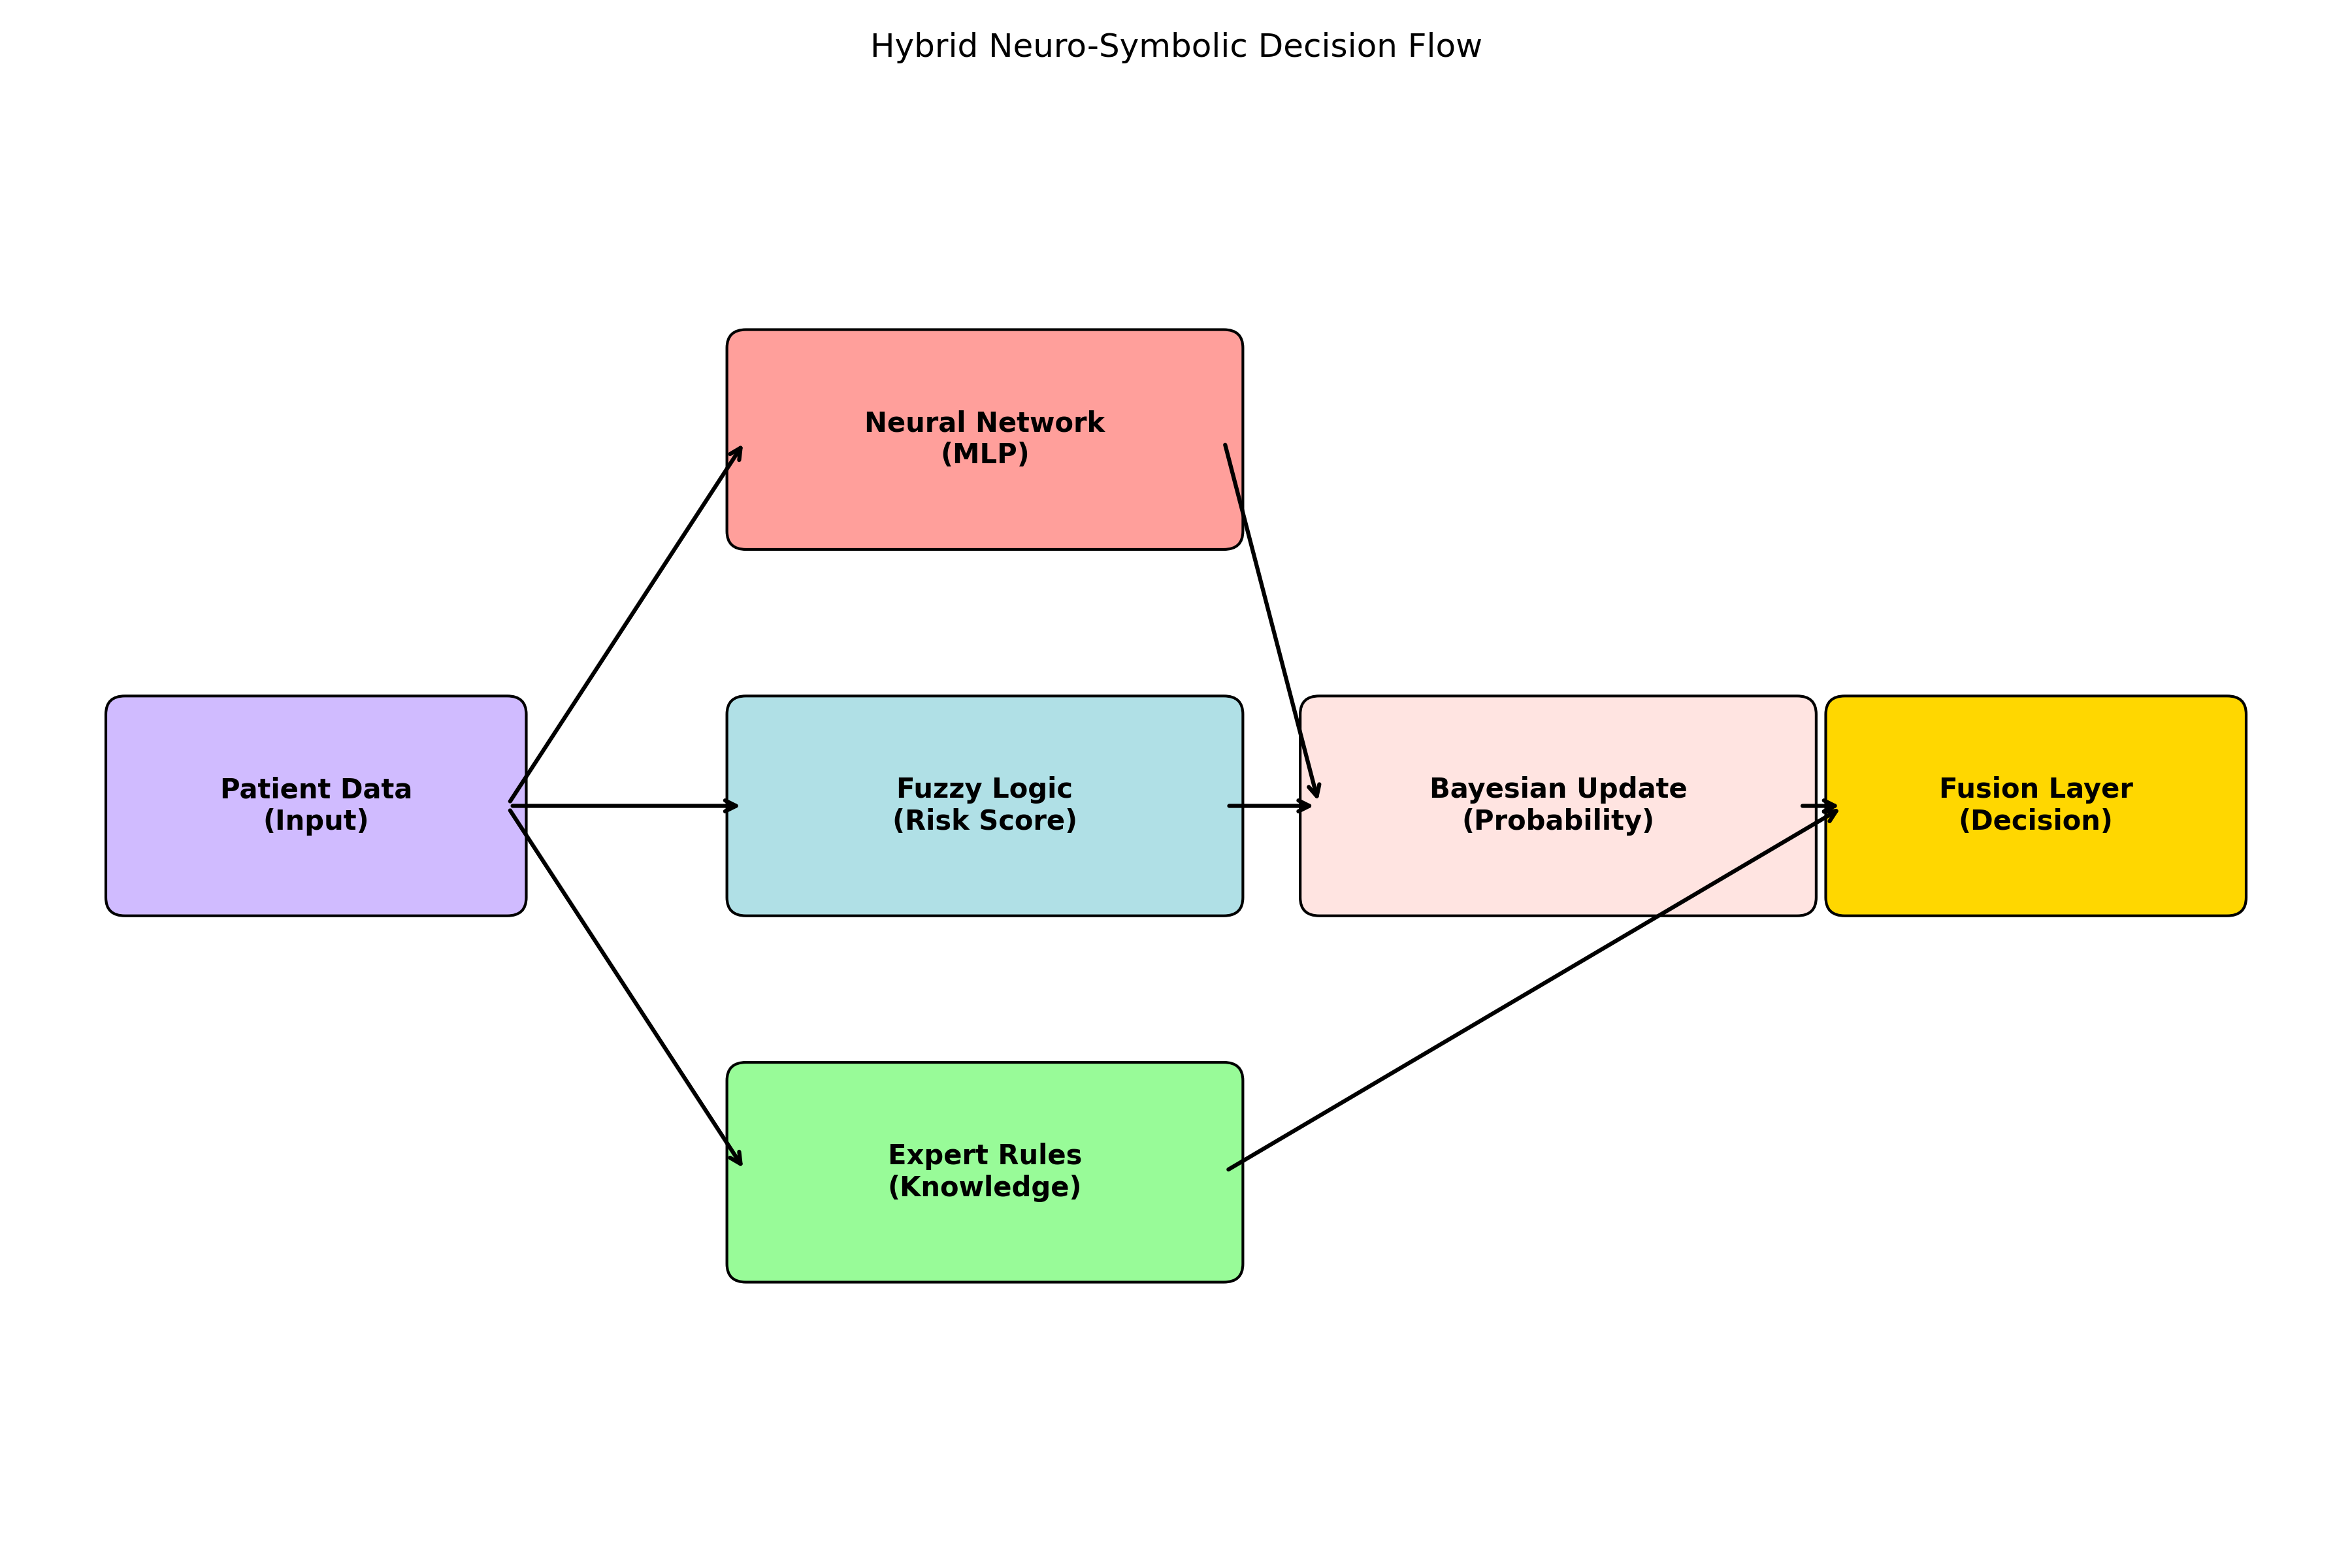
\includegraphics[width=0.95\linewidth]{figures/hybrid_flow.png}}
\caption{Hybrid Neuro-Symbolic Decision Flow.}
\label{fig:hybrid_flow}
\end{figure}

\section{Experiments & Results}

\subsection{Performance & HPO Convergence}
We evaluated models using Accuracy, Precision, Recall, F1, and ROC-AUC. Figure \ref{fig:hpo_convergence} shows Optuna converging fastest ($ROC \approx 0.83$). Table \ref{tab:hpo_comparison} confirms Optuna and Enhanced ALSHADE as top performers.

\input{generated_tables/table_baselines.tex}

\begin{figure}[htbp]
\centerline{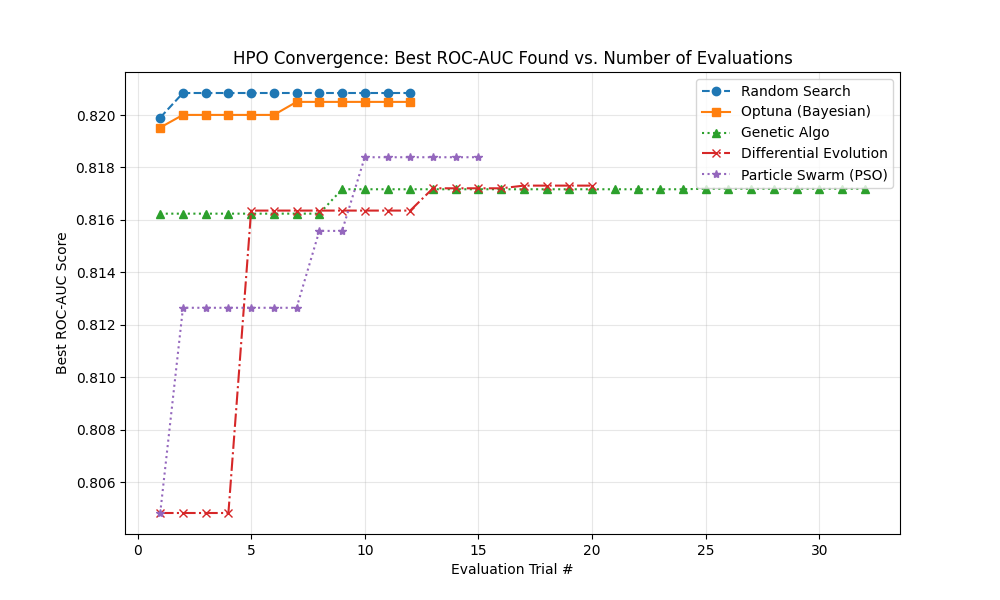
\includegraphics[width=0.9\linewidth]{figures/hpo_convergence.png}}
\caption{HPO Convergence: Optuna vs. GA vs. Random.}
\label{fig:hpo_convergence}
\end{figure}

\input{generated_tables/table_optimizers.tex}

Hyperparameter distributions (Figs. \ref{fig:hpo_distributions}, \ref{fig:hpo_dist_iso}) show that the "Total Defense" pipeline stabilizes performance across the search space.

\begin{figure}[htbp]
\centerline{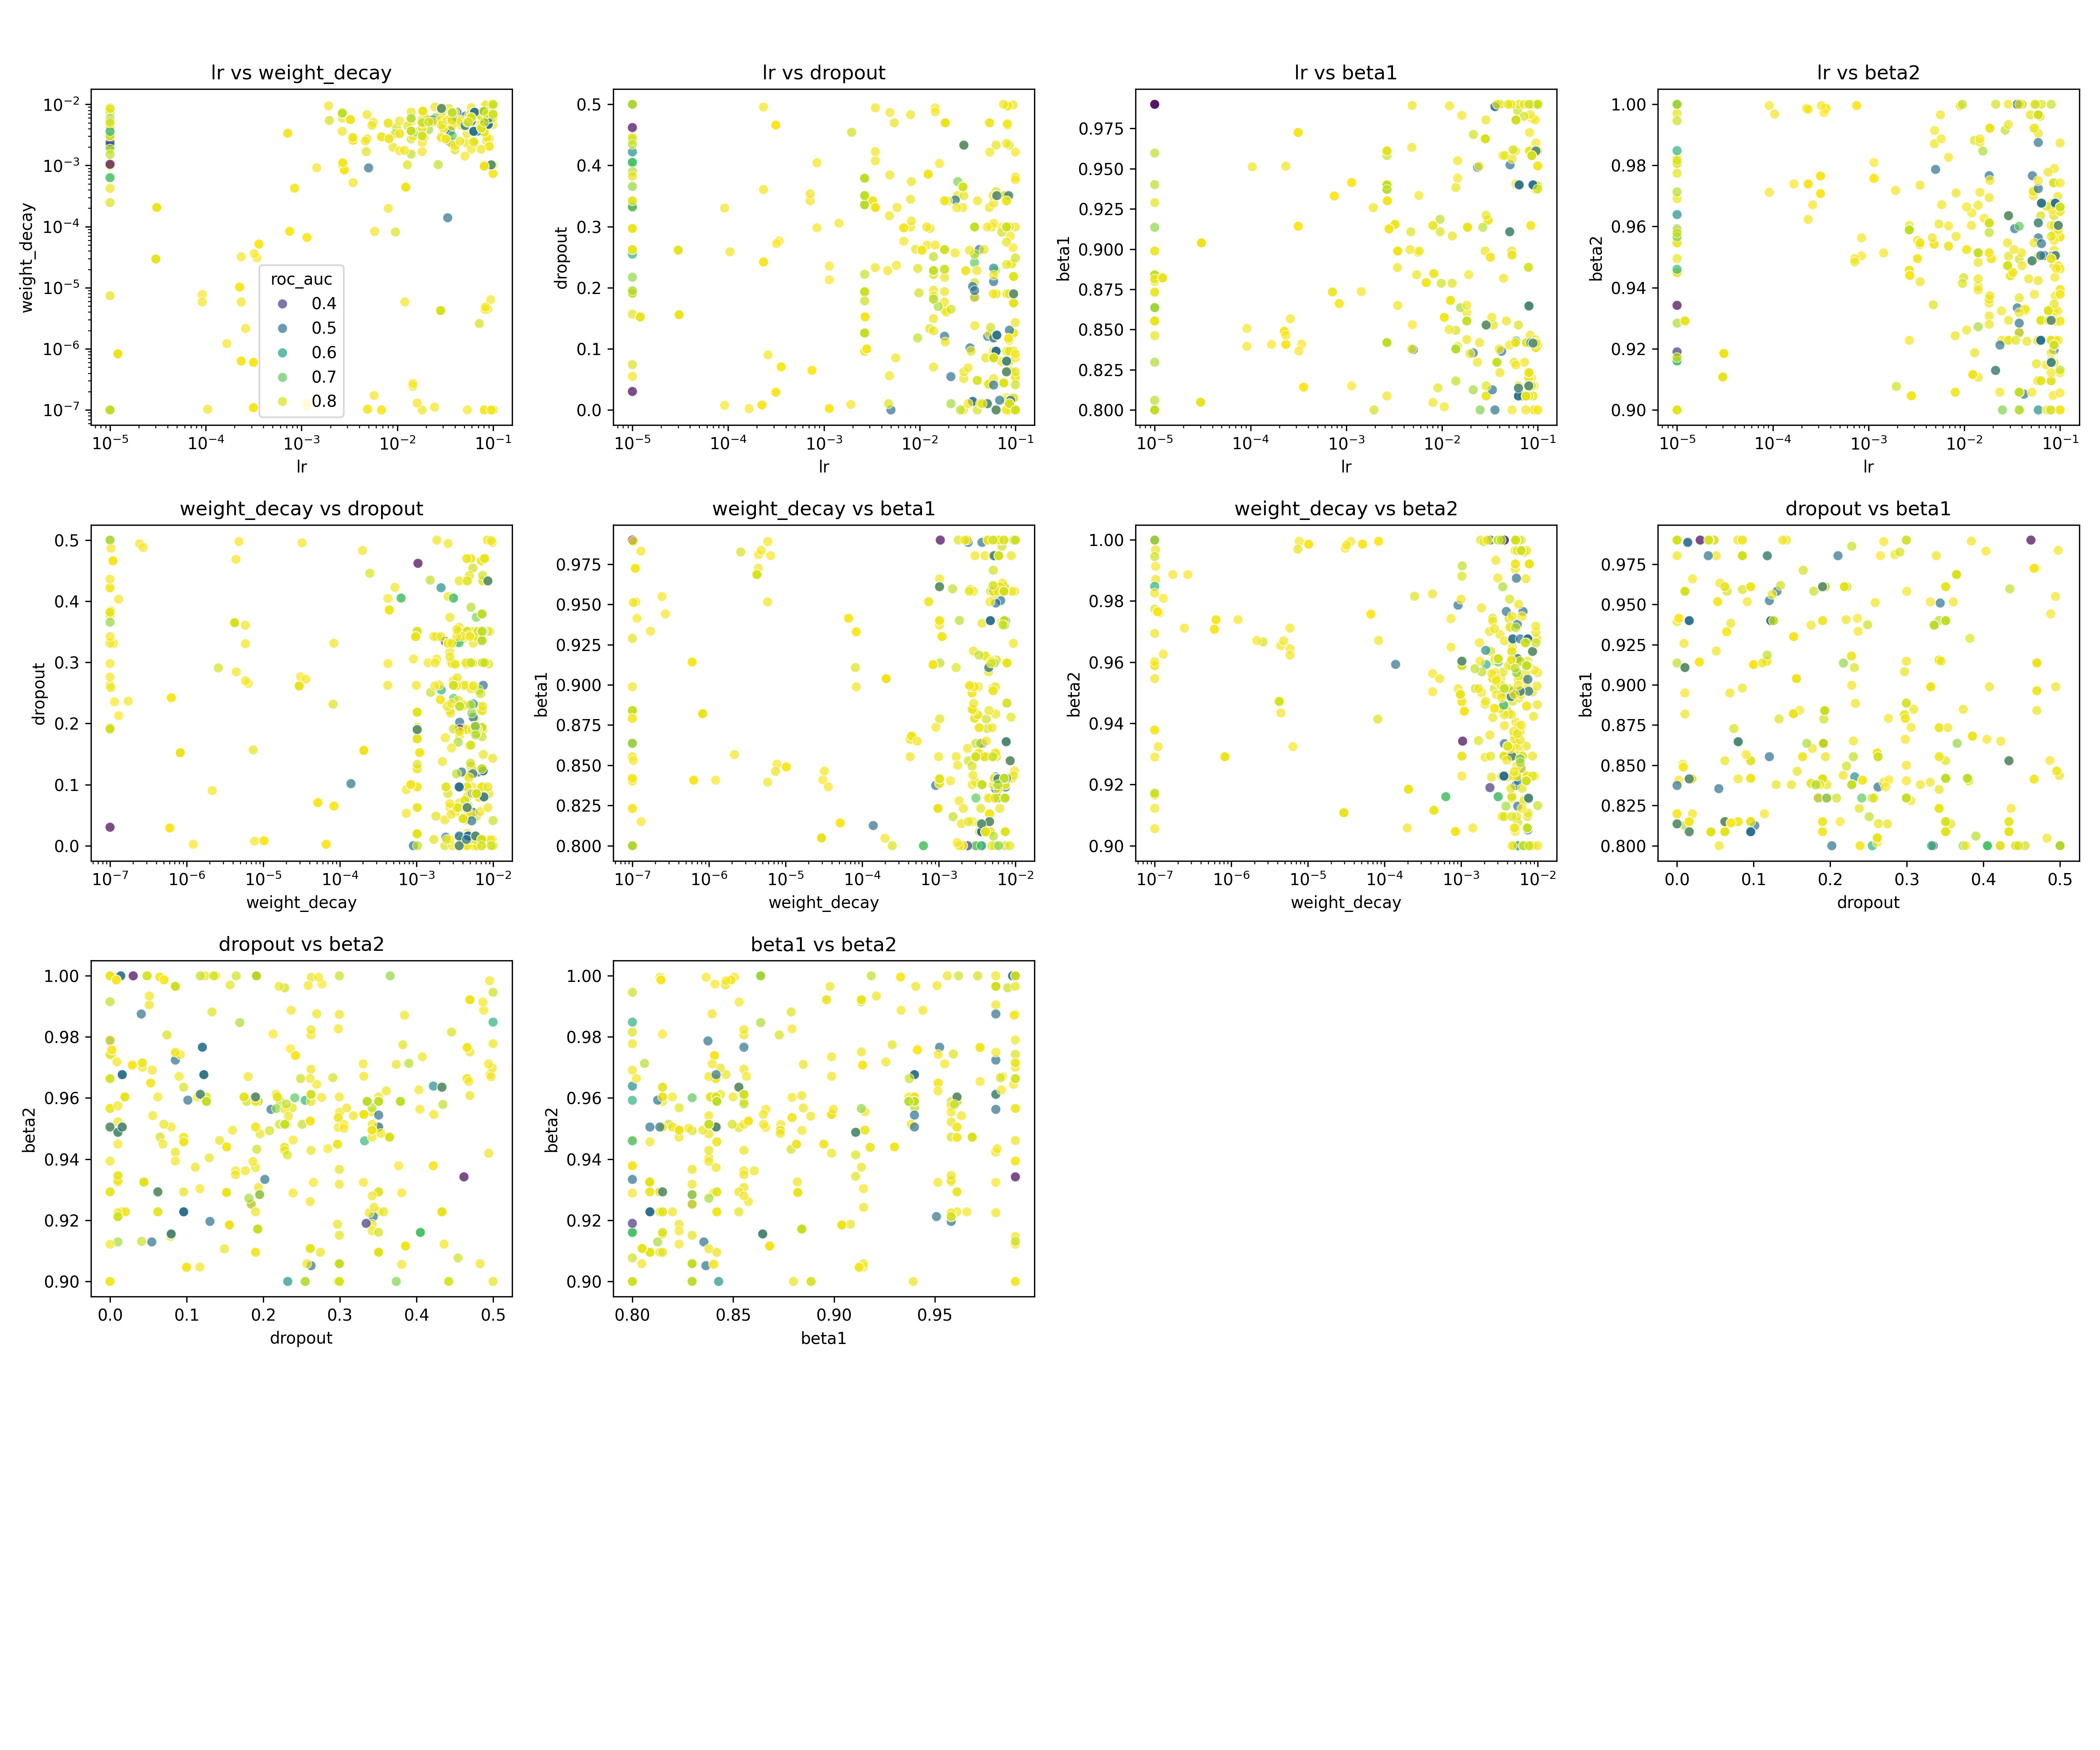
\includegraphics[width=1.0\linewidth]{figures/hpo_distributions_iso.png}}
\caption{Hyperparameter Distributions (Isolation Forest).}
\label{fig:hpo_dist_iso}
\end{figure}

\begin{table}[htbp]
\caption{HPO Comparison}
\begin{center}
\begin{tabular}{|l|c|c|}
\hline
\textbf{Method} & \textbf{Best ROC-AUC} & \textbf{Time (s)} \\
\hline
Random Search & 0.8286 & 176.5 \\
Bayesian (Optuna) & \textbf{0.8322} & 2143.5 \\
Genetic Algorithm & 0.8252 & 1140.5 \\
Enhanced ALSHADE & 0.8264 & 1984.2 \\
\hline
\end{tabular}
\label{tab:hpo_comparison}
\end{center}
\end{table}

\subsection{Calibration & Analysis}
The optimized MLP shows good calibration (Fig. \ref{fig:reliability}) and appropriately shifts risk for borderline BMI/Age cases (Figs. \ref{fig:borderline_bmi}, \ref{fig:borderline_age}). Feature importance (Fig. \ref{fig:feature_importance}) confirms reliance on valid medical factors like General Health and BMI.

\input{generated_tables/table_representation.tex}

\begin{figure}[htbp]
\centerline{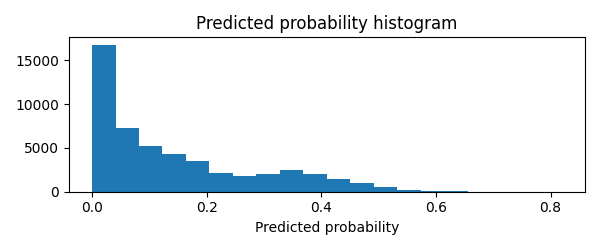
\includegraphics[width=0.9\linewidth]{figures/reliability_diagram.png}}
\caption{Reliability Diagram.}
\label{fig:reliability}
\end{figure}

\begin{figure}[htbp]
\centerline{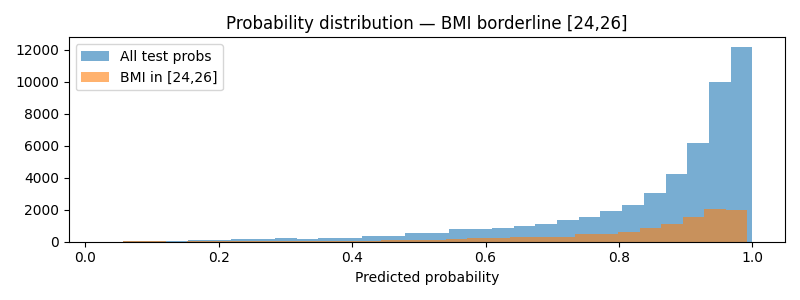
\includegraphics[width=0.9\linewidth]{figures/borderline_bmi.png}}
\caption{Borderline BMI analysis.}
\label{fig:borderline_bmi}
\end{figure}

\begin{figure}[htbp]
\centerline{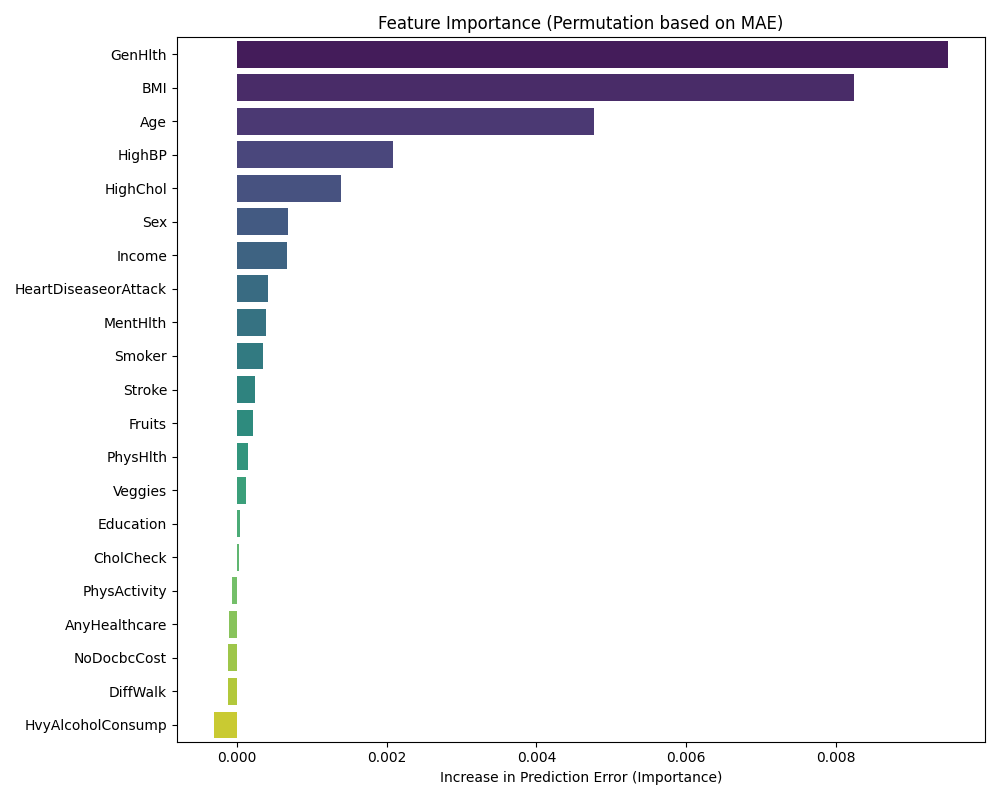
\includegraphics[width=0.9\linewidth]{figures/feature_importance.png}}
\caption{Permutation Feature Importance.}
\label{fig:feature_importance}
\end{figure}

\subsection{Neuro-Symbolic Validation}
Table VI and Table \ref{tab:auditing} highlight the system's safety. While the MLP achieved higher raw AUC (0.82 vs 0.79), the Hybrid system recovered **2,245 False Negatives** (20.36\% reduction).

\begin{table}[htbp]
\caption{Hard False Negatives Analysis}
\begin{center}
\begin{tabular}{|c|c|c|c|c|}
\hline
\textbf{ID} & \textbf{True} & \textbf{MLP} & \textbf{Fuzzy} & \textbf{Bayes} \\
\hline
46974 & 1 & 0.0005 & 0.0476 & 0.0000 \\
5789 & 1 & 0.0013 & 0.0435 & 0.0000 \\
\hline
\end{tabular}
\label{tab:hard_examples}
\end{center}
\end{table}

\input{generated_tables/table_auditing.tex}

The ablation study (Figs. \ref{fig:ablation_heatmap}-\ref{fig:roc_comparison}) confirms that the fuzzy-Bayesian layer provides crucial robustness.

\begin{figure}[htbp]
\centerline{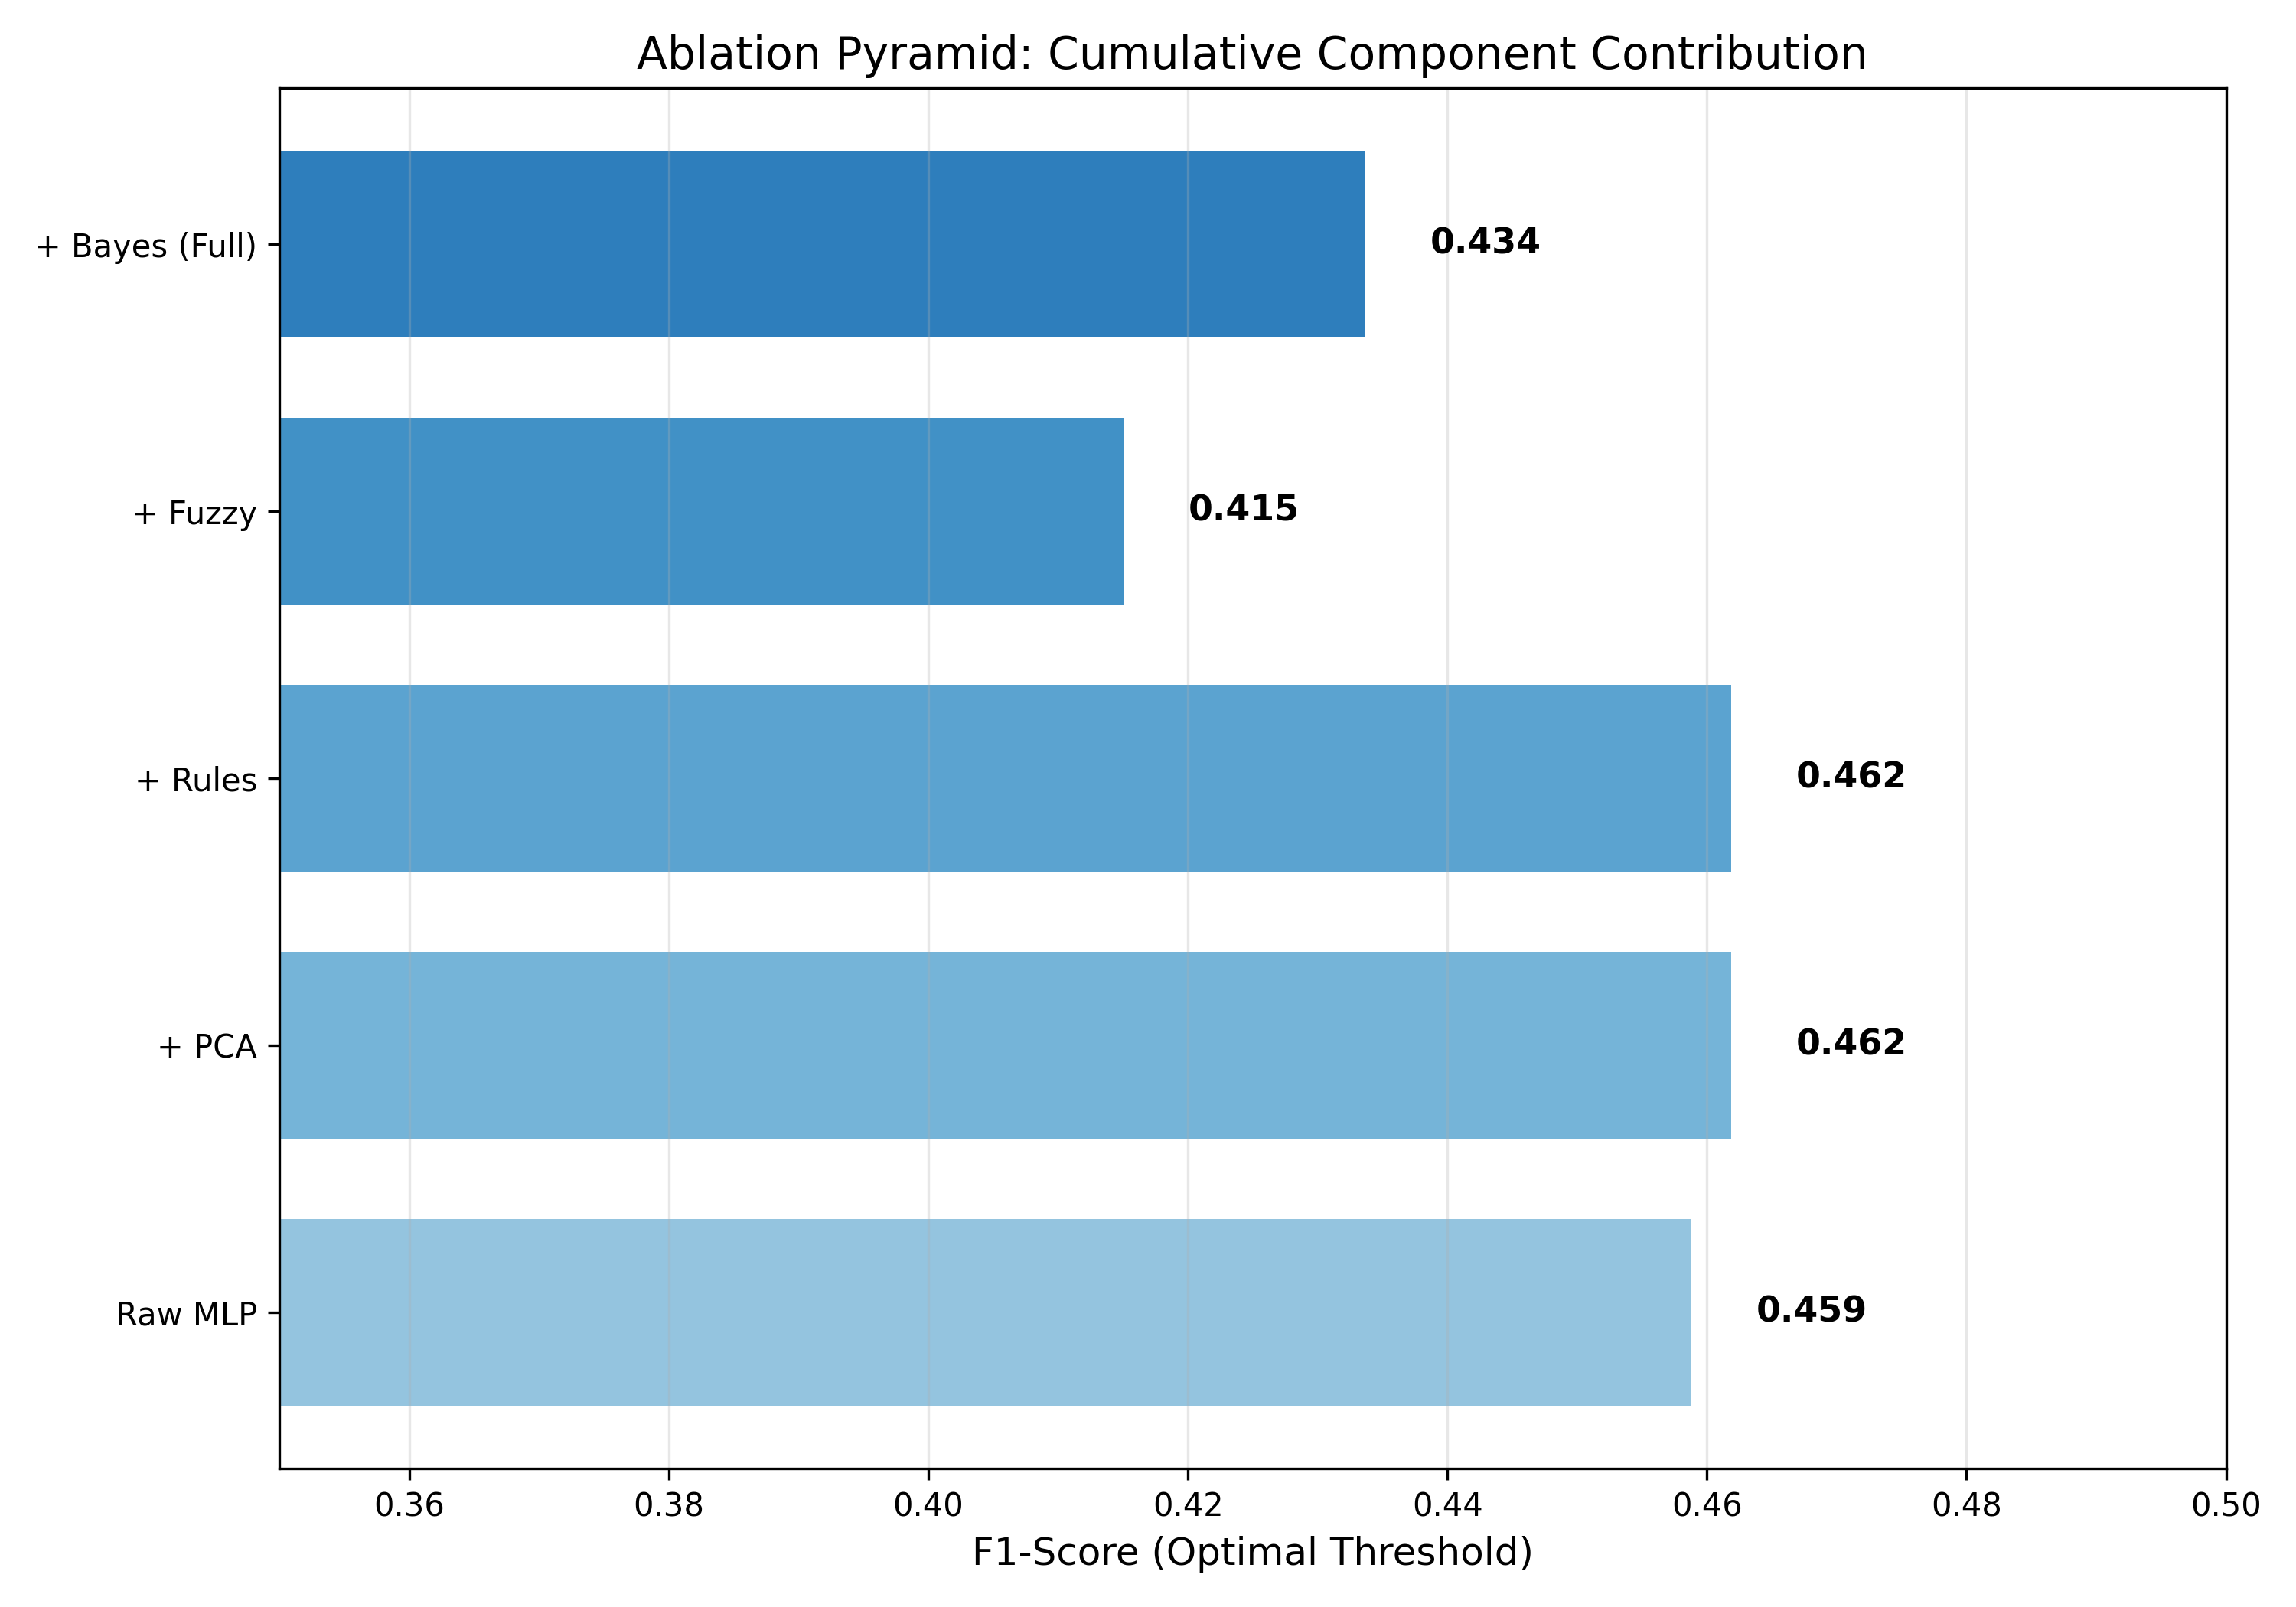
\includegraphics[width=0.8\linewidth]{figures/ablation_pyramid.png}}
\caption{Ablation Pyramid.}
\label{fig:ablation_pyramid}
\end{figure}

\begin{figure}[htbp]
\centerline{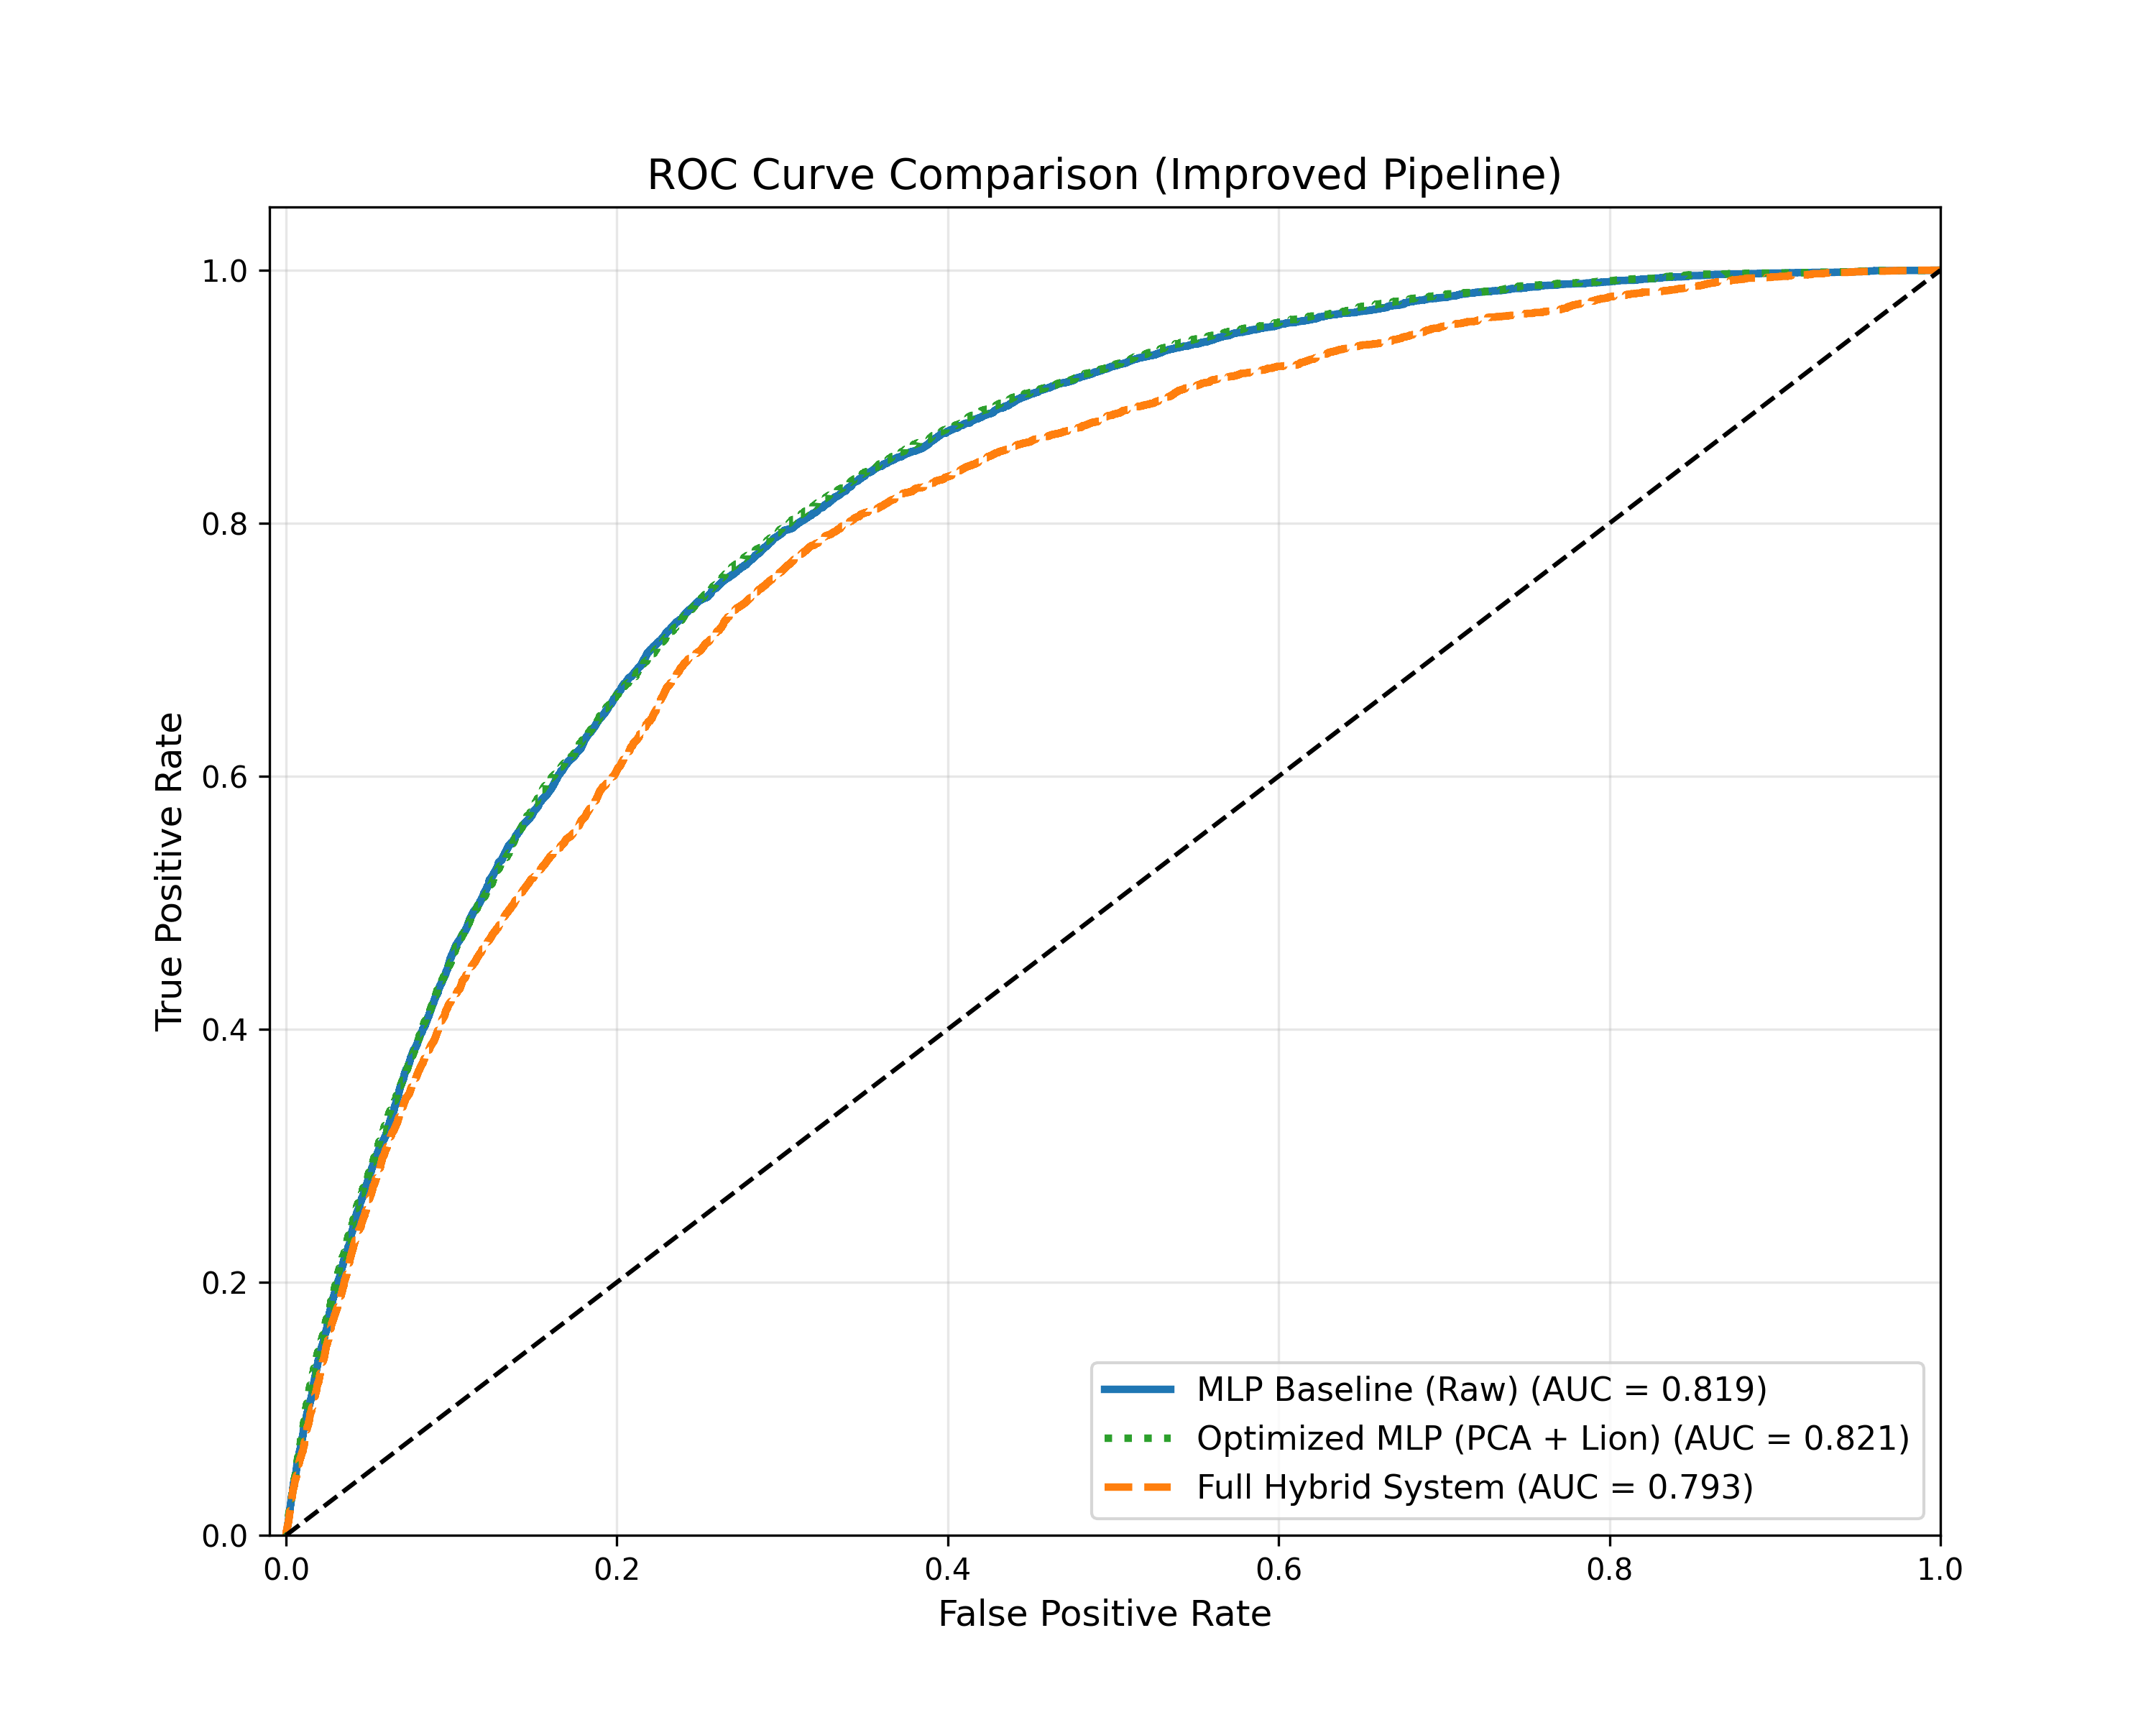
\includegraphics[width=0.9\linewidth]{figures/roc_curves_comparison.png}}
\caption{ROC Curve: MLP vs. Hybrid.}
\label{fig:roc_comparison}
\end{figure}

\section{Conclusion}
We optimized a deep learning baseline to a peak **ROC-AUC of 0.8212** (PCA + Lion). However, by integrating a Neuro-Symbolic safety layer, we traded slight statistical discrimination (0.79 AUC) for a **20\% reduction in missed diagnoses**. This "Total Defense" approach demonstrates that hybrid AI can function as an effective safety net, validating the potential for trustworthy, human-in-the-loop medical systems.

\section*{Appendix: Reproducibility}
**Rules:** 1) Obese&Old $\rightarrow$ High Risk. 2) HighBP&Chol $\rightarrow$ High Risk. 3) Sedentary $\rightarrow$ High Risk. 4) Frail $\rightarrow$ High Risk. 5) Healthy $\rightarrow$ Low Risk.
**Fuzzy Sets:** BMI Low/Med/High; Age Young/Mid/Old (Triangular functions).
**HPO Budgets:** 15 trials (Random/Optuna); 32 evals (Evolutionary).

\bibliographystyle{IEEEtran}
\bibliography{references}

\section*{Supplementary Material}

\begin{table*}[t]
\centering
\scriptsize
\caption{Hyperparameter Optimization (HPO) Strategy Analysis for Raw Input (ISO)}
\label{tab:opt_raw_iso}
\begin{tabular}{llllllllllll}
\toprule 
\textbf{Feature} & \textbf{Optimizer} & \textbf{HPO Method} & \textbf{Acc} & \textbf{Prec} & \textbf{Rec} & \textbf{F1} & \textbf{ROC} & \textbf{Epochs} & \textbf{Run-Time} & \textbf{$p$-value} & \textbf{F-Rank}  \\
\midrule
\multirow{24}{*}{ Raw Input} & \multirow{4}{*}{ RMSProp} & Random Search & 0.7880 & 0.3487 & 0.6011 & 0.4413 & 0.8036 & 15 & 211.9s & n.s. & 21 \\
 &  & Bayesian Opt. & 0.8014 & 0.3661 & 0.5816 & 0.4493 & 0.8094 & 66 & 4926.3s & < 0.001 & 14 \\
 &  & Genetic Algo. & 0.7821 & 0.3456 & 0.6312 & 0.4466 & 0.8096 & 36 & 1329.5s & < 0.001 & 13 \\
 &  & ALSHADE & 0.8025 & 0.3690 & 0.5881 & 0.4534 & 0.8136 & 26 & 1749.3s & n.s. & 6 \\
\cline{2-12}
 & \multirow{4}{*}{ Adam} & Random Search & 0.8020 & 0.3702 & 0.5999 & 0.4578 & 0.8150 & 15 & 189.5s & < 0.001 & 4 \\
 &  & Bayesian Opt. & 0.7901 & 0.3534 & 0.6108 & 0.4478 & 0.8083 & 64 & 2332.0s & < 0.001 & 16 \\
 &  & Genetic Algo. & 0.7850 & 0.3494 & 0.6302 & 0.4495 & 0.8108 & 36 & 1654.2s & < 0.001 & 11 \\
 &  & ALSHADE & 0.8064 & 0.3726 & 0.5692 & 0.4504 & 0.8111 & 22 & 2355.1s & < 0.001 & 10 \\
\cline{2-12}
 & \multirow{4}{*}{ SGD} & Random Search & 0.7941 & 0.3599 & 0.6141 & 0.4538 & 0.8149 & 15 & 228.6s & < 0.001 & 5 \\
 &  & Bayesian Opt. & 0.7994 & 0.3675 & 0.6104 & 0.4588 & 0.8193 & 71 & 2565.1s & < 0.001 & 1 \\
 &  & Genetic Algo. & 0.7998 & 0.3665 & 0.5990 & 0.4547 & 0.8157 & 32 & 1140.5s & < 0.001 & 3 \\
 &  & ALSHADE & 0.7900 & 0.3504 & 0.5941 & 0.4408 & 0.8065 & 32 & 1651.1s & < 0.001 & 18 \\
\cline{2-12}
 & \multirow{4}{*}{ Adagrad} & Random Search & 0.7998 & 0.3602 & 0.5629 & 0.4393 & 0.8026 & 15 & 187.5s & < 0.001 & 22 \\
 &  & Bayesian Opt. & 0.7802 & 0.3422 & 0.6261 & 0.4426 & 0.8045 & 28 & 2155.9s & < 0.001 & 19 \\
 &  & Genetic Algo. & 0.8030 & 0.3685 & 0.5804 & 0.4508 & 0.8129 & 32 & 1859.8s & < 0.001 & 8 \\
 &  & ALSHADE & 0.7924 & 0.3544 & 0.5968 & 0.4447 & 0.8078 & 50 & 1984.2s & < 0.001 & 17 \\
\cline{2-12}
 & \multirow{4}{*}{ Adadelta} & Random Search & 0.8022 & 0.3677 & 0.5835 & 0.4511 & 0.8100 & 15 & 197.8s & < 0.001 & 12 \\
 &  & Bayesian Opt. & 0.7945 & 0.3589 & 0.6040 & 0.4503 & 0.8090 & 23 & 1449.4s & < 0.001 & 15 \\
 &  & Genetic Algo. & 0.8067 & 0.3753 & 0.5824 & 0.4565 & 0.8171 & 32 & 1591.7s & < 0.001 & 2 \\
 &  & ALSHADE & 0.7830 & 0.3409 & 0.5970 & 0.4340 & 0.8011 & 60 & 2427.9s & < 0.001 & 23 \\
\cline{2-12}
 & \multirow{4}{*}{ Lion} & Random Search & 0.7873 & 0.3527 & 0.6306 & 0.4524 & 0.8119 & 15 & 176.5s & < 0.001 & 9 \\
 &  & Bayesian Opt. & 0.7950 & 0.3604 & 0.6089 & 0.4528 & 0.8135 & 74 & 1980.7s & < 0.001 & 7 \\
 &  & Genetic Algo. & 0.6264 & 0.2405 & 0.7790 & 0.3675 & 0.7175 & 36 & 1199.0s & < 0.001 & 24 \\
 &  & ALSHADE & 0.7888 & 0.3508 & 0.6067 & 0.4446 & 0.8043 & 28 & 1265.0s & < 0.001 & 20 \\
\bottomrule
\end{tabular}
\end{table*}

\begin{table*}[t]
\centering
\scriptsize
\caption{Hyperparameter Optimization (HPO) Strategy Analysis for PCA (ISO)}
\label{tab:opt_pca_iso}
\begin{tabular}{llllllllllll}
\toprule 
\textbf{Feature} & \textbf{Optimizer} & \textbf{HPO Method} & \textbf{Acc} & \textbf{Prec} & \textbf{Rec} & \textbf{F1} & \textbf{ROC} & \textbf{Epochs} & \textbf{Run-Time} & \textbf{$p$-value} & \textbf{F-Rank}  \\
\midrule
\multirow{24}{*}{ PCA} & \multirow{4}{*}{ RMSProp} & Random Search & 0.8132 & 0.3845 & 0.5670 & 0.4583 & 0.8202 & 15 & 175.4s & n.s. & 8 \\
 &  & Bayesian Opt. & 0.8004 & 0.3690 & 0.6096 & 0.4597 & 0.8207 & 62 & 2143.5s & < 0.001 & 3 \\
 &  & Genetic Algo. & 0.8013 & 0.3697 & 0.6043 & 0.4588 & 0.8168 & 36 & 1198.2s & < 0.001 & 19 \\
 &  & ALSHADE & 0.7925 & 0.3609 & 0.6347 & 0.4602 & 0.8198 & 26 & 1726.2s & < 0.001 & 14 \\
\cline{2-12}
 & \multirow{4}{*}{ Adam} & Random Search & 0.8133 & 0.3845 & 0.5664 & 0.4581 & 0.8204 & 15 & 192.1s & < 0.001 & 5 \\
 &  & Bayesian Opt. & 0.8073 & 0.3765 & 0.5840 & 0.4579 & 0.8188 & 71 & 2335.8s & < 0.001 & 17 \\
 &  & Genetic Algo. & 0.7953 & 0.3630 & 0.6214 & 0.4583 & 0.8189 & 36 & 1053.0s & < 0.001 & 16 \\
 &  & ALSHADE & 0.7994 & 0.3680 & 0.6124 & 0.4597 & 0.8201 & 58 & 1419.6s & < 0.001 & 12 \\
\cline{2-12}
 & \multirow{4}{*}{ SGD} & Random Search & 0.8066 & 0.3763 & 0.5903 & 0.4596 & 0.8202 & 15 & 155.0s & < 0.001 & 7 \\
 &  & Bayesian Opt. & 0.7747 & 0.3368 & 0.6366 & 0.4405 & 0.8037 & 77 & 2111.3s & < 0.001 & 23 \\
 &  & Genetic Algo. & 0.8061 & 0.3756 & 0.5915 & 0.4594 & 0.8206 & 32 & 853.1s & < 0.001 & 4 \\
 &  & ALSHADE & 0.7074 & 0.2600 & 0.5960 & 0.3621 & 0.7288 & 37 & 1395.3s & < 0.001 & 24 \\
\cline{2-12}
 & \multirow{4}{*}{ Adagrad} & Random Search & 0.8126 & 0.3839 & 0.5700 & 0.4588 & 0.8201 & 15 & 171.1s & < 0.001 & 13 \\
 &  & Bayesian Opt. & 0.7962 & 0.3645 & 0.6223 & 0.4597 & 0.8196 & 60 & 2093.5s & < 0.001 & 15 \\
 &  & Genetic Algo. & 0.7973 & 0.3656 & 0.6188 & 0.4596 & 0.8202 & 32 & 1388.6s & < 0.001 & 11 \\
 &  & ALSHADE & 0.7862 & 0.3548 & 0.6526 & 0.4597 & 0.8202 & 45 & 3700.5s & < 0.05 & 6 \\
\cline{2-12}
 & \multirow{4}{*}{ Adadelta} & Random Search & 0.7958 & 0.3627 & 0.6154 & 0.4564 & 0.8174 & 25 & 557.3s & < 0.001 & 18 \\
 &  & Bayesian Opt. & 0.7944 & 0.3595 & 0.6089 & 0.4521 & 0.8125 & 46 & 1585.8s & < 0.001 & 21 \\
 &  & Genetic Algo. & 0.8112 & 0.3824 & 0.5770 & 0.4599 & 0.8211 & 32 & 2705.8s & < 0.001 & 2 \\
 &  & ALSHADE & 0.7915 & 0.3605 & 0.6415 & 0.4616 & 0.8202 & 13 & 3026.5s & < 0.001 & 10 \\
\cline{2-12}
 & \multirow{4}{*}{ Lion} & Random Search & 0.7935 & 0.3613 & 0.6281 & 0.4587 & 0.8202 & 29 & 514.2s & < 0.001 & 9 \\
 &  & Bayesian Opt. & 0.8048 & 0.3749 & 0.6012 & 0.4619 & 0.8212 & 47 & 1388.2s & < 0.001 & 1 \\
 &  & Genetic Algo. & 0.7794 & 0.3448 & 0.6482 & 0.4502 & 0.8081 & 36 & 2528.1s & < 0.001 & 22 \\
 &  & ALSHADE & 0.8016 & 0.3693 & 0.5992 & 0.4570 & 0.8157 & 49 & 1979.9s & < 0.05 & 20 \\
\bottomrule
\end{tabular}
\end{table*}

\begin{table*}[t]
\centering
\scriptsize
\caption{Hyperparameter Optimization (HPO) Strategy Analysis for Autoencoder (ISO)}
\label{tab:opt_ae_iso}
\begin{tabular}{llllllllllll}
\toprule 
\textbf{Feature} & \textbf{Optimizer} & \textbf{HPO Method} & \textbf{Acc} & \textbf{Prec} & \textbf{Rec} & \textbf{F1} & \textbf{ROC} & \textbf{Epochs} & \textbf{Run-Time} & \textbf{$p$-value} & \textbf{F-Rank}  \\
\midrule
\multirow{24}{*}{ Autoencoder} & \multirow{4}{*}{ RMSProp} & Random Search & 0.7871 & 0.3038 & 0.4087 & 0.3485 & 0.6793 & 14 & 510.2s & n.s. & 19 \\
 &  & Bayesian Opt. & 0.7609 & 0.3013 & 0.5427 & 0.3875 & 0.7473 & 71 & 1538.9s & < 0.001 & 8 \\
 &  & Genetic Algo. & 0.7225 & 0.2789 & 0.6258 & 0.3859 & 0.7489 & 36 & 2906.0s & < 0.001 & 7 \\
 &  & ALSHADE & 0.5618 & 0.2072 & 0.7591 & 0.3256 & 0.6906 & 49 & 0.0s & < 0.001 & 17 \\
\cline{2-12}
 & \multirow{4}{*}{ Adam} & Random Search & 0.7847 & 0.3014 & 0.4139 & 0.3488 & 0.7079 & 15 & 565.4s & < 0.001 & 16 \\
 &  & Bayesian Opt. & 0.7643 & 0.3018 & 0.5265 & 0.3837 & 0.7423 & 71 & 1649.7s & < 0.001 & 12 \\
 &  & Genetic Algo. & 0.7154 & 0.2799 & 0.6629 & 0.3936 & 0.7537 & 36 & 2415.2s & < 0.001 & 3 \\
 &  & ALSHADE & 0.7533 & 0.2945 & 0.5526 & 0.3843 & 0.7540 & 34 & 3086.2s & < 0.001 & 2 \\
\cline{2-12}
 & \multirow{4}{*}{ SGD} & Random Search & 0.7706 & 0.2915 & 0.4518 & 0.3544 & 0.7223 & 25 & 470.4s & < 0.001 & 14 \\
 &  & Bayesian Opt. & 0.7939 & 0.3123 & 0.3988 & 0.3503 & 0.7170 & 71 & 1320.0s & < 0.001 & 15 \\
 &  & Genetic Algo. & 0.7141 & 0.2769 & 0.6529 & 0.3889 & 0.7530 & 36 & 2571.5s & < 0.001 & 4 \\
 &  & ALSHADE & 0.7415 & 0.2816 & 0.5511 & 0.3727 & 0.7442 & 44 & 0.0s & < 0.001 & 11 \\
\cline{2-12}
 & \multirow{4}{*}{ Adagrad} & Random Search & 0.7310 & 0.2805 & 0.5947 & 0.3812 & 0.7516 & 25 & 901.1s & < 0.001 & 5 \\
 &  & Bayesian Opt. & 0.1393 & 0.1393 & 1.0000 & 0.2446 & 0.4555 & 46 & 1795.0s & < 0.001 & 23 \\
 &  & Genetic Algo. & 0.7490 & 0.3007 & 0.6046 & 0.4016 & 0.7552 & 32 & 3316.5s & < 0.001 & 1 \\
 &  & ALSHADE & 0.1393 & 0.1393 & 1.0000 & 0.2446 & 0.4239 & 30 & 4257.3s & < 0.001 & 24 \\
\cline{2-12}
 & \multirow{4}{*}{ Adadelta} & Random Search & 0.7345 & 0.2806 & 0.5791 & 0.3781 & 0.7458 & 25 & 1119.4s & < 0.001 & 10 \\
 &  & Bayesian Opt. & 0.1393 & 0.1393 & 1.0000 & 0.2446 & 0.4574 & 46 & 2484.8s & < 0.001 & 22 \\
 &  & Genetic Algo. & 0.7479 & 0.2922 & 0.5690 & 0.3861 & 0.7499 & 32 & 3151.6s & < 0.001 & 6 \\
 &  & ALSHADE & 0.7477 & 0.2854 & 0.5391 & 0.3732 & 0.7462 & 58 & 3659.1s & < 0.001 & 9 \\
\cline{2-12}
 & \multirow{4}{*}{ Lion} & Random Search & 0.7872 & 0.3042 & 0.4098 & 0.3492 & 0.6617 & 15 & 1106.6s & < 0.001 & 20 \\
 &  & Bayesian Opt. & 0.7731 & 0.3083 & 0.5054 & 0.3830 & 0.7284 & 46 & 2373.2s & < 0.001 & 13 \\
 &  & Genetic Algo. & 0.6889 & 0.2525 & 0.6287 & 0.3602 & 0.6864 & 36 & 3789.4s & < 0.001 & 18 \\
 &  & ALSHADE & 0.1393 & 0.1393 & 1.0000 & 0.2446 & 0.5000 & 60 & 3813.3s & < 0.001 & 21 \\
\bottomrule
\end{tabular}
\end{table*}

\end{document}
